% options:
% thesis=B bachelor's thesis
% thesis=M master's thesis
% czech thesis in Czech language
% slovak thesis in Slovak language
% english thesis in English language
% hidelinks remove colour boxes around hyperlinks

\documentclass[thesis=M,czech,hidelinks]{FITthesis}[2012/06/26]

\usepackage[utf8]{inputenc} % LaTeX source encoded as UTF-8

\usepackage{multirow} % multirow for tabular
\usepackage{graphicx} %graphics files inclusion
\usepackage{amsmath} %advanced maths
\usepackage{amssymb} %additional math symbols

\usepackage{algorithm}
\usepackage{algpseudocode}
\usepackage{dirtree} %directory tree visualisation
% \usepackage{textcomp} % \textcopyleft

% % list of acronyms
% \usepackage[acronym,nonumberlist,toc,numberedsection=autolabel]{glossaries}
% \iflanguage{czech}{\renewcommand*{\acronymname}{Seznam pou{\v z}it{\' y}ch zkratek}}{}
% \makeglossaries
\newcommand{\tg}{\mathop{\mathrm{tg}}} %cesky tangens
\newcommand{\cotg}{\mathop{\mathrm{cotg}}} %cesky cotangens
\newcommand{\0}{{\textcolor[gray]{0.75}{0}}}

\newsubfloat{figure}

\newenvironment{algoritmus}{
    \floatname{algorithm}{Algoritmus}
    \begin{algorithm}
}{\end{algorithm}}

\newtheorem{tvrzeni}{Tvrzení}
\newtheorem{definice}{Definice}
\newtheorem{veta}{Věta}

% % % % % % % % % % % % % % % % % % % % % % % % % % % % % %
% Hlavička
% % % % % % % % % % % % % % % % % % % % % % % % % % % % % %

\department{Katedra počítačových systémů}
\title{Asymetrický šifrovací algoritmus McEliece}
\authorGN{Vojtěch}
\authorFN{Myslivec}
\authorWithDegrees{Bc. Vojtěch Myslivec}
\supervisor{prof. Ing. Róbert Lórencz, CSc.}
\website{https://github.com/VojtechMyslivec/mceliece-mathematica}

%\acknowledgements{Rodina, Lórencz, Kalvoda, Kotil, Guth} %TODO
\abstractCS{Tady bude nejaky kuuul abstakt } %TODO
\abstractEN{Sem doplňte ekvivalent abstraktu Vaší práce v~angličtině.} %TODO
\placeForDeclarationOfAuthenticity{V~Praze}
\declarationOfAuthenticityOption{4} %volba Prohlášení (číslo 1-6)
\keywordsCS{McEliece, asymetrická kryptografie, postkvantová kryptografie,
binární Goppa kódy, konečná tělesa, polynomy, Wolfram Mathematica}
\keywordsEN{McEliece, public-key cryptography, post-quantum cryptography, binary
Goppa codes, finite fields, polynomials, Wolfram Mathematica}




% % % % % % % % % % % % % % % % % % % % % % % % % % % % % %
% Dokument
% % % % % % % % % % % % % % % % % % % % % % % % % % % % % %

\begin{document}

% \newacronym{CVUT}{{\v C}VUT}{{\v C}esk{\' e} vysok{\' e} u{\v c}en{\' i} technick{\' e} v Praze}
% \newacronym{FIT}{FIT}{Fakulta informa{\v c}n{\' i}ch technologi{\' i}}

% ====================================================================
% ====================================================================
% ====================================================================
\begin{introduction}

% TODO

Tato práce se zabývá asymetrickým kryptosystémem \emph{McEliece}. Mezi největší
přednosti tohoto systému patří jeho odolnost vůči kvantovým počítačům a je tak
jedním z~vhodných kandidátů pro asymetrickou kryptografii pro postkvantovou
dobu.

V~prvních kapitolách této práce jsou popsány nezbytné primitivy z~oblasti
matematiky a teorie kódování, které jsou potřeba pro pochopení a použití
kryptosystému McEliece. Jedná se především o~počítání s~\emph{konečnými tělesy}
a \emph{polynomy} (kapitola \ref{kap_telesa}) a binární \emph{Goppa} kódy
(kapitola \ref{kap_kody}).

Kryptosystému \emph{McEliece} se věnuje kapitola \ref{kap_mceliece}. Kromě
základního popisu generování klíčů a algoritmů pro šifrování a dešifrování je
probráno i kryptosystém \emph{Niederreiter} -- \uv{úprava} kryptosystému
\emph{McEliece} pro získání \emph{digitálního podpisu}. Jsou ukázány slabiny,
nevýhody i možné útoky na kryptosystém McEliece a též zmíněna praktická varianta
systému odolná vůči těmto aspektům.

V~poslední části  práce je probrána implementace kryptosystému \emph{McEliece}
v~softwaru \emph{Wolfram Mathematica} včetně změřených časových
% TODO a prostorových
složitostí (kapitola \ref{kap_implementace}).

\end{introduction}





% ====================================================================
% ====================================================================
% ====================================================================
\chapter{Obecná algebra}\label{kap_telesa}

V~této kapitole uvedeme pojmy a algoritmy nutné pro práci s~\emph{konečnými
tělesy} a \emph{polynomy} nad konečnými tělesy (\emph{rozšířená tělesa}). Při
popisu je předpokládána znalost základních pojmů z~oblasti \emph{algebry},
zejména \emph{lineární}. Definice byly převzaty z~\cite{Paar,Mares,Pytlicek}
a~tuto literaturu zároveň doporučujeme pro hlubší studium této problematiky.

\paragraph{Poznámka:} Algoritmy zmíněné v~následujících kapitolách jsou detailně
-- včetně pseudokódu -- popsány v~kapitole~\ref{kap_implementace}, která se
zabývá konkrétní implementací algoritmů a operací.



% ====================================================================
\section{Základní termíny}

Pro ujasnění je uvedena definice tělesa:

\begin{definice}[Těleso]
    Nechť $M$ je neprázdná množina a $+$ a $\cdot$ binární operace\footnote{
        Pro zjednodušení zápisu je $\cdot$ často vynecháváno.
    }. Struktura
    $T=\big(M, +, \cdot \big)$ se nazývá těleso, pokud platí
    \begin{enumerate}
        \item $\big(M, +\big)$ je \emph{komutativní grupa} (nazývána
            \emph{aditivní})
        \item $\big(M\setminus\{\mathit{0}\}, \cdot \big)$\footnote{
                Prvek $\mathit{0}$ je \emph{nulový} (\emph{neutrální}) prvek
                \emph{aditivní grupy}.
            } je \emph{grupa} (nazývána
            \emph{multiplikativní})
        \item Platí (levý i pravý) \emph{distributivní zákon}:
            $$
                \forall a,b,c \in M :
                \big( a(b+c) = a b + a c \big) \land
                \big( (b+c)a = b a + c a \big)
            $$

    \end{enumerate}
\end{definice}
\emph{Těleso}, které má konečný počet prvků, se nazývá \emph{konečné těleso}.

\begin{veta}
    Nechť $T$ je \emph{konečné těleso}, pak jeho počet prvků (\emph{řád}) je
    $p^n$, kde $p$ je prvočíslo a $n \in \mathbb{N} \land n \geq 1 $.
\end{veta}

Číslo $p$ se nazývá \emph{charakteristika}. Navíc platí, že \emph{všechna
konečná tělesa} se stejným počtem prvků jsou navzájem \emph{izomorfní}.
\emph{Konečné těleso} řádu $p^n$ je tedy dále označováno jako $GF(p^n)$
(z~anglického \emph{Gallois field}, dle francouzského matematika \emph{Évariste
Galois}).



% ====================================================================
\section{Reprezentace prvků}

Jak ukážeme dále, je vhodné prvky konečného tělesa $GF(p^n)$ reprezentovat jako
\emph{polynomy} s~koeficienty z~množiny $\mathbb{Z}_p=\{0,1,\ldots,p-1\}$, tedy
prvek $a \in GF(p^n)$ lze zapsat:
$$
    A(x) = \sum_{i=0}^{n-1} a_i x^i, a_i \in \mathbb{Z}_p
$$
O~takovém polynomu říkáme, že je to \emph{polynom nad tělesem $GF(p)$ (stupně
maximálně $n-1$)}. Na prvek $a$ se je možné dívat též jako na vektor či $n$-tici
koeficientů~$a_i$:
$$
    A(x) \cong a \cong (a_{n-1} a_{n-2} \ldots a_0) \cong
    a_{n-1} a_{n-2} \ldots a_0
$$

V~této práci budeme mezi těmito reprezentacemi nadále volně přechází, jak bude
v~daném kontextu potřeba\footnote{
    V~některých materiálech se používá i obráceného zápisu
    $(a_0 a_1 \ldots a_{n-1})$.
}.



% ====================================================================
\section{Operace v~tělese $GF(p^n)$}

V~následujících sekcích uvedeme operace potřebné pro počítání s~tělesy
$GF(p^n)$. Konkrétní zvolené algoritmy a~jejich implementace je detailně popsána
v~kapitole~\ref{kap_implementace}.

\paragraph{Poznámka:} Kvůli zobecnění definic budeme v~této podkapitole používat
označení tělesa $GF(p)$ jako těleso~$\mathbb{F}$.


% --------------------------------------------------------------------
\subsection{Sčítání}

Sčítání v~tělese $GF(p^n)$ je definováno stejně jako sčítání polynomů, s~tím, že
sčítání jednotlivých koeficientů je prováděno \emph{modulo $p$} (v~tělese
$GF(p)$:
$$
    A(x) + B(x) = \sum a_i x^i + \sum b_i x^i =
    \sum \left|a_i + b_i\right|_p x^i
$$


% --------------------------------------------------------------------
\subsection{Násobení}

Násobení v~tělese $GF(p^n)$ nelze provádět \uv{po složkách}, jako je tomu
u~sčítání. U~takto definované operace by většina prvků neměla (multiplikativní)
\emph{inverzi} a~nejednalo by se tak o~\emph{těleso}.

Při násobení prvků opět využijeme jejich reprezentace pomocí polynomů.
Výsledkem násobení pak je:
$$
    A(x) \cdot B(x) = \sum_{i=0}^{n-1} a_i x^i \cdot \sum_{i=0}^{n-1} b_i x^i =
    \sum_{i=0}^{2n-2} \left|\sum_{j+k=i} a_j \cdot b_k\right|_p x^i
$$

Jak je naznačeno, násobení i sčítání koeficientů se provádí \emph{modulo} $p$
(respektive v~tělese~$\mathbb{F}$).

Kvůli uzavřenosti násobení v~tělese je nutné zavést operaci \uv{zbytek po dělení
polynomu} $A(x)$ polynomem $P(x)$, neboli $A(x) \mod P(x)$. Navíc pro pro
jednoznačné určení tělesa $GF(p^n)$ je třeba určit příslušný \emph{ireducibilní}
polynom $P(x)$, který bude použitý při operaci násobení modulo $P(x)$.

\begin{definice}
    Polynom $P(x)$ nad tělesem $GF(p)$ je \emph{ireducibilní} právě tehdy, když
    pro každé dva polynomy $A(x)$ a $B(x)$ nad $GF(p)$ platí:
    $$
        A(x) \cdot B(x) = P(x) \Rightarrow \left( deg(A(x)) = 0 \right) \lor
        \left( deg(B(x)) = 0 \right)
    $$
\end{definice}

Jinými slovy pro \emph{ireducibilní} polynom platí, že tento polynom nelze
rozložit na polynomy nad~$\mathbb{F}$ stupně větší než~$1$.

\paragraph{Příklad} Polynom $x^3+x+1$ je nad tělesem $GF(2)$
\emph{ireducibilní}, protože neexistuje jeho rozklad na polynomy stupně alespoň
$1$. Polynom $x^2+1$ není nad tělesem $GF(2)$ \emph{ireducibilní}, protože:
$$ (x+1)\cdot(x+1) = x^2 + \left|1+1\right|_2x + 1 = x^2+1 $$

Nyní je možné zavést operaci násobení dvou prvků tělesa jako násobení dvou
polynomů \emph{modulo} \emph{zadaný ireducibilní} polynom:
$$
    A(x) \cdot B(x) = \sum a_i x^i \cdot \sum b_i x^i =
    \sum \left|\sum_{j+k=i} a_j \cdot b_k\right|_p x^i \mod P(x)
$$

\paragraph{Poznámka:} Pokud by zvolený $P(x)$ nebyl \emph{ireducibilní}, jednalo
by se o~\emph{okruh}, nikoliv o~\emph{těleso}, protože by neexistovala
\emph{multiplikativní inverze} pro některé prvky a~navíc by i~existovaly tzv.
\emph{dělitelé nuly}.


% --------------------------------------------------------------------
\subsection{Umocňování}

Pro rozšíření operací o~opakované násobení je vhodné zavést operaci umocňování.

\begin{definice}
    Nechť $a$ je prvkem (libovolného) tělesa $T$ a číslo $n\in\mathbb{N}$. Operace
    umocňování definujeme následovně:
    \begin{align*}
        a^0     &= 1 \\
        a^n     &= \underbrace{a \cdot a \cdot \ldots \cdot a}_{\text{$n$-krát}} \\
        a^{-n}  &= \left(a^{-1}\right)^n
    \end{align*}
\end{definice}

Pro efektivní výpočet mocniny prvku je vhodné použít algoritmus
\emph{Square-and-Multiply}, kde se dílčí operace \uv{square} a~\uv{multiply}
provádí operací $\cdot$ v~daném tělese $F$.


% --------------------------------------------------------------------
\subsection{Inverze}

\emph{Inverzi} v~\emph{grupě} lze obecně definovat následovně:

\begin{definice}[Inverze]
    Nechť $G = (M,\circ)$ je \emph{grupa}, $a$ jejím prvkem a~$\mathbb{O}$ jejím
    neutrálním prvkem. Prvek $\bar{a}$ je \emph{inverzí} prvku $a$, pokud platí
    následující rovnice:
    $$ a \circ \bar{a} = \mathbb{O} $$
\end{definice}

\paragraph{Aditivní inverze} \hfil \\
Inverze v~\emph{aditivní grupě} značíme znaménkem minus \uv{$-$} a~je z~definice
velmi triviální:
$$
    \left| A(x) + (-A(x)) \right|_p = 0 \Rightarrow -A(x) =
    \sum \left|-a_i\right|_p x^i
$$

Neboli je to aditivní inverze jednotlivých koeficientů \emph{modulo}~$p$
(v~tělese~$F$).


\paragraph{Multiplikativní inverze} \hfil \\
Inverze v~\emph{multiplikativní grupě} značíme záporným exponentem~\uv{$^{-1}$}
či symbolem dělení.
$$
    \left| A(x) \cdot A(x)^{-1} \right|_{P(x)} =
    \left| \frac{A(x)}{A(x)} \right|_{P(x)} =
    \mathbf{1}
$$

Tuto \emph{multiplikativní inverzi} je třeba počítat \emph{rozšířeným Euklidovým
algoritmem pro polynomy} (\emph{EEA}), či případně jinými algoritmy, jako je
například \emph{algoritmus Itoh-Teechai-Tsujii} (\emph{ITT}) \cite{FIT_BHW,ITT}.

\emph{Rozšířený Euklidův algoritmus} \emph{pro polynomy}, stejně jako
v~modulární aritmetice (neboli pro tělesa $GF(p)$), stojí na nalezení
\emph{Bézoutovy rovnosti}. Pro výpočet \emph{EEA} je třeba výpočtu dělení
polynomů se zbytkem\footnote{
    Někdy uváděno jako dlouhé dělení.
}, nicméně v~binárních tělesech lze toto dělení nahradit prostým posouváním
a~\uv{odečítáním} (respektive sčítáním) prvků.



% ====================================================================
\section{Rozšířená tělesa}
V~algebře se dá rozšíření těles definovat velmi obecně. Pro účely naší práce
nás ale budou ve své podstatě zajímat pouze tělesa $GF(2^n)^m$.

\begin{definice}{Rozšíření tělesa:}
    Nechť $T$ je těleso a~$P$ podmnožina množiny tělesa $T$. Pokud $P$ tvoří
    (s~původními operacemi) opět těleso, říkáme, že $P$ je \emph{podtělesem}~$T$
    a~zároveň $T$ je \emph{rozšířením} tělesa $P$.
\end{definice}


\paragraph{Polynomy jako rozšířená tělesa} \hfil \\
Na konečná tělesa $GF(p^n)$ realizované polynomy, jak byly představeny v~minulé
kapitole je možné se dívat jako na \emph{rozšíření} tělesa $GF(2)$. Stejně tak,
jako jsme sestrojily polynomy nad $GF(2^n)$ (\uv{polynomy nad polynomy}).

\begin{definice}{Okruh polynomů:}
    Nechť $\mathbb{F}$ je těleso. Množinu okruhu polynomů $R = \mathbb{F}[x]$
    definujeme jako všechny polynomy s~koeficienty z~tělesa $\mathbb{F}$
    a~operace tohoto okruhu jako klasické operace s~polynomy s~tím, že operace
    s~koeficienty jsou prováděny v~tělese $\mathbb{F}$.
\end{definice}

Tato definice jistě dává smysl, protože operace v~tělese $\mathbb{F}$ jsou
\emph{uzavřené} a~výsledkem sčítání respektive násobení dvou polynomů
z~$\mathbb{F}[x]$ vznikne polynom, který opět patří do tohoto okruhu.

V~případě zavedení operace \emph{modulo polynom} můžeme zavést násobení stejným
způsobem, jako bylo uvedeno v~předešlé kapitole.

\begin{tvrzeni}
    Nechť $\mathbb{F}$ je konečné těleso a~$g \in \mathbb{F}[x]$ \emph{ireducibilní}
    polynom stupně~$n$. Potom množina všech polynomů z~$\mathbb{F}[x]$ stupně
    menší než $t$ tvoří s~klasickou operací s~polynomy $+$ a~s~násobením
    modulo~$g$ \emph{konečné těleso} $\mathbb{F}^n$.\footnote{
        Toto těleso se dá též značit jako (faktorokruh) $\mathbb{F}[x]/(g)$, kde
        $(g)$ je \emph{ideál} generovaný polynomem $g$.
    }
\end{tvrzeni}

V~této práci budeme nadále používat termín \emph{rozšířené těleso} ve smyslu
konečného tělesa reprezentované polynomy s~koeficienty z~tělesa $GF(2^m)$.
Rozšířením tak získáme těleso $GF(2^m)^n$.\footnote{
    Toto těleso je izomorfní s~tělesem  $GF(2^{mn})$.
}


\paragraph{Poznámka:} Pokud rozšířením konečného tělesa vnikne opět konečné
těleso (dle tvrzení výše), je možné toto těleso opět rozšířit a~induktivním
krokem tak rozšiřovat tělesa do libovolné \uv{hloubky}. Jinými slovy polynomy
s~operací modulo (ireducibilní) polynom tvoří opět těleso a~jdou tak využít jako
koeficienty dalších polynomů.


\paragraph{Použité značení} \hfil \\
Příklady počítání operací v~těchto \emph{rozšířených} tělesech jsou uvedeny
v~kapitole implementace~\ref{kap_implementace_teles}. Pro ujasnění způsobu
značení prvků z~těchto těles zde uvedeme příklad tohoto značení.

Máme těleso $\mathbb{F} = GF(2^3)$ s~ireducibilním polynomem
$$  g(y) = y^3 + y + 1$$
Tento polynom budeme zkráceně zapisovat jako $1011$. Potom polynom~$a$
z~okru\-hu~$\mathbb{F}[x]$ zapisujeme těmito ekvivalentními způsoby:
\begin{align*}
    a(x) &= (y^2 + 1)x^3 + (y)x + (y+1)         \cong \\
         &\cong (101)x^3 + (010)x + (011) \quad \cong \\
         &\cong (101)(000)(010)(011)
\end{align*}





% ====================================================================
% ====================================================================
% ====================================================================
\chapter{Teorie kódování}\label{kap_kody}

V~této kapitole definujeme a~vysvětlíme pojmy z~teorie kódování, které jsou
použité v~kryptosystému \emph{McEliece} (kapitola~\ref{kap_mceliece}). Definice
byly čerpané z~\cite{FIT_AAK,Adamek} a~pro další studium této problematiky je
též doporučeno~\cite{McEliece_coding}.

V~podkapitolách uvádíme základní značení a~termíny z~oblasti samoopravných
(\ref{kap_samoopravne_kody}) a~lineárních (\ref{kap_linearni_kody}) kódů.
V~poslední kapitole~\ref{kap_goppa_kody} se věnujeme \emph{binárním Goppa
kódům}, které jsou přímo použité v~kryptosystému \emph{McEliece}.

% ====================================================================
\section{Samoopravné kódy}\label{kap_samoopravne_kody}

Teorie kódování spadá do oblasti teorie informace a zabývá se způsoby
\emph{zakódování} či \emph{reprezentací} zpráv a~jejich přenosem.

V~této kapitole budeme používat následujícího značení (odpovídá
obrázku~\ref{obr_kodovani}):

\begin{center}
\begin{tabular}{l p{10cm}}
    $+$     &   binární bitová operace \emph{XOR} \\
    $-$     &   inverzní operace k~$+$, tedy též \emph{XOR} \\
    $a$     &   zpráva délky $k$ \\
    $K()$   &   operace \emph{zakódování} \\
    $b$     &   zakódovaná zpráva délky $n$; $b=K(a)$ a zpravidla platí $n>k$ \\
    $e$     &   chybový vektor délky $n$ vzniklý při přenosu $b$ \\
    $c$     &   přijatá zpráva ($c=b+e$) \\
    $D()$   &   operace dekódování \\
    $d$     &   \emph{dekódovaná} zpráva; $d=D(c)$ \\
    $s$     &   \emph{syndrom} přijaté zprávy/chyby (viz dále) délky $r$;
                zpravidla platí $r=n-k$ \\
\end{tabular}
\end{center}

\begin{figure}
    \centering
    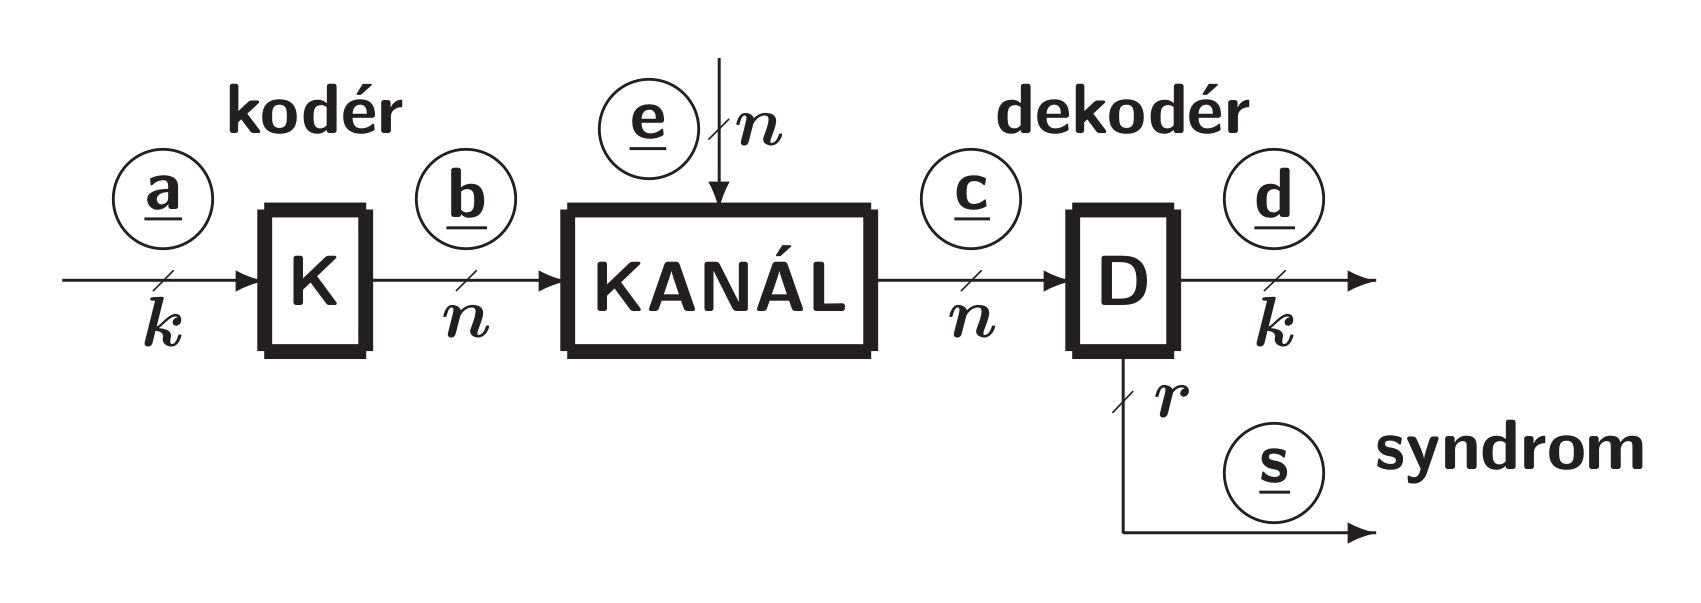
\includegraphics[width=0.8\textwidth]{materialy/aak-kodovani.png}
    \caption{Použité značení při kódování~\cite{FIT_AAK}}
    \label{obr_kodovani}
\end{figure}


\begin{definice}{(Binární) kód:}
    Nechť existuje (prosté) zobrazení $\mathcal{K}$ z~množiny všech možných
    zpráv $a$ délky $k$ do množiny kódových slov $b$ délky $n$
    ($GF(2)^k \rightarrow GF(2)^n$). Pak toto zobrazení nazveme
    kódem~$\mathcal{K}$ s~parametry $(n,k)$.\footnote{
        Obecně lze \emph{kód} definovat jako zobrazení $\mathcal{L}^k
        \rightarrow \mathcal{M}^n$, kde $\mathcal{L}$ je \emph{abeceda} zpráv
        délky $k$ a~$\mathcal{M}$ abeceda kódových slov délky $n$.
    }
\end{definice}

\paragraph{Poznámka:} V~této práci nadále předpokládáme použití pouze
\emph{blokových kódů} (dle definice). Dají se definovat i~kódy s~proměnlivou
délkou kódových slov.

Z~definice prostého zobrazení vyplývá, že existuje \emph{kódové slovo} pro
\emph{všechny} zprávy a~že existuje \emph{inverzní} zobrazení
$\mathcal{K}^{-1}$. Množina všech kódových slov je jednoznačně určena zobrazením
množiny zpráv $\mathcal{B} = \mathcal{K}(GF(2)^k) = \mathcal{K}(\mathcal{A})$.
Vektory délky $n$, které nepatří do množiny $\mathcal{B}$ nazveme jako
\emph{nekódová slova} (vektory). Operací \emph{zakódování} budeme rozumět
aplikaci zobrazení $\mathcal{K}$ a~operací dekódování aplikaci
$\mathcal{K}^{-1}$, tedy získání původní zprávy z~(\emph{kódového}) slova.

\begin{definice}{Hammingova vzdálenost:}
    \emph{Hammingova vzdálenost} dvou vektorů $u$ a~$v$ -- $vzd(u,v)$ či
    $H(u,v)$ -- je počet rozdílných \emph{bitů} ve vektorech $u$~a~$v$:
    $vzd(u,v) = \sum \left| u_i - v_i \right|$
\end{definice}

\emph{Hammingovu váhu} vektoru $v$ pak definujeme jako \emph{Hammingovu
vzdálenost} vektoru $v$ od \emph{nulového vektoru} patřičné délky. Jinými slovy
je to počet \emph{nenulových} bitů (\uv{jedniček}) vektoru $v$.
$$ H(v) = H(v,\mathbf{0}) $$


\begin{definice}{Kódová vzdálenost:}
    Kódová vzdálenost kódu $\mathcal{K}$ je minimální \emph{Hammingova
    vzdálenost} mezi všemi kódovými slovy.
    $$
        kvzd(\mathcal{K}) =
        \min_{\substack{\forall b1,b2 \in \mathcal{B} \\ b1 \neq b2}} vzd(b1,b2)
    $$
\end{definice}

Dále budeme značit $d = kvzd(\mathcal{K})$. Pokud je~$d > 1$, tak je jasné, že
můžeme za jistých okolností odhalit (detekovat), že při přenosu kódového slova
nastala chyba. Pokud by ale nastalo~$d$~a~více chyb, je možné, aby se z~jednoho
\emph{kódového slova} stalo \emph{kódové slovo} jiné (viz příklad
s~\emph{Hammingovými} kódy v~kapitole~\ref{kap_hammingovy_kody}).

\paragraph{Detekční kód} \hfil \\
Kód, který dokáže při dekódování zjistit, že při přenosu nastala chyba nazýváme
kódem \emph{detekčním}. Při kódové vzdálenosti~$d$ je z~principu možné
detekovat~$d-1$ chyb.

\paragraph{Samoopravný kód} \hfil \\
Kód, který dokáže při dekódování dokáže opravit chybu (způsobenou přenosem),
nazýváme kódem \emph{samoopravným}. Při kódové vzdálenosti $d$ je z~principu
možné opravit~$t = \lfloor \frac{d-1}{2} \rfloor$~chyb. Operace
\emph{dekódování} potom z~nekódového slova dokáže nalézt nejbližší (ve smyslu
\emph{Hammingově vzdálenosti}) slovo \emph{kódové}. U~samoopravných kódů uvádíme
parametry včetně počtu chyb, které kód dokáže opravit, tedy $(n,k,t)$\footnote{
    V~některých zdrojích se místo počtu opravitelných chyb objevuje kódová
    vzdálenost, tedy~$(n,k,d)$, což odpovídá~$(n,k,2t+1)$.
}.


Počet opravitelných chyb naznačují obrázky~\ref{obr_kvzd}. Vrcholy úseček
představují vektory délky~$n$ mezi dvěma kódovými slovy~$b_1$ a~$b_2$ (naznačení
nejkratší \emph{kódové vzdálenosti} v~prostoru $GF(2^n)$). V~případě, že~$d$ je
liché~\ref{obr_kvzd_licha}, vždy existuje jednoznačný nejbližší vektor. V~případě,
že~$d$ je sudé~\ref{obr_kvzd_suda}, tak pokud přijatý vektor~$c$ leží přesně
uprostřed mezi dvěma nejbližšími vektory, není možné rozhodnout, na které kódové
slovo by se měl vektor~$c$ dekódovat.

\begin{figure}
    \centering
    \subbottom[Příklad liché $kvzd$\label{obr_kvzd_licha}]{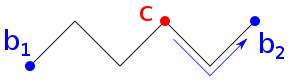
\includegraphics[width=0.45\textwidth]{materialy/kvzd_licha.png}}
    \quad
    \subbottom[Příklad sudé $kvzd$\label{obr_kvzd_suda}]{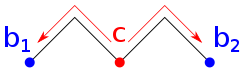
\includegraphics[width=0.38\textwidth]{materialy/kvzd_suda.png}}
    \caption{Ilustrace problému nalezení nejbližšího kódového slova \label{obr_kvzd}}
\end{figure}

Existuje několik kategorií \emph{samoopravných} kódů. Definice kategorie kódu ve
své podstatě určuje, jakým způsobem bude probíhat konstrukce kódu (respektive
kódového slova), aby se zajistila určitá kódová vzdálenost~$d$ a~při dekódování
bylo možné nalézt patřičný počet chyb $t$.

V~této práci budeme nadále pracovat pouze se \emph{samoopravnými kódy}.



% ====================================================================
\section{Lineární kódy}\label{kap_linearni_kody}
Dalším důležitým pojmem, který budeme v~práci používat jsou \emph{lineární
kódy}.

\begin{definice}{Lineární kód:}
    Nechť je zobrazení odpovídající kódu $\mathcal{K}$ \emph{lineární},
    pak nazýváme tento kód \emph{lineárním}.
\end{definice}

Jinými slovy \emph{kódová slova} kódu $\mathcal{K}$ tvoří \emph{lineární
prostor} -- přesněji \emph{lineární podprostor} vektorového prostoru $GF(2)^n$.
V~tomto prostoru definujeme klasické operace sčítání dvou vektorů jako operaci
\emph{XOR} a~násobení skaláru s~vektorem jako operaci násobení po jednotlivých
složkách vektoru. Je jasné, že v~případě násobení skalárem $0$ je výsledek
operace násobení skalárem \emph{nulový vektor} ($0 \cdot \mathbf{v} = \mathbf{0}$)
a~násobením skalárem $1$ získáme původní (nezměněný) vektor
($1 \cdot \mathbf{v} = \mathbf{v}$).

Z~definice lineárního prostoru též plyne, že \emph{nulový vektor}~$\mathbf{0}$
je vždy kódovým slovem \emph{lineárního} kódu $\mathcal{K}$.

\begin{tvrzeni}
    Kódová vzdálenost lineárního kódu $\mathcal{K}$ odpovídá minimální váze ze
    všech kódových slov (kromě nulového vektoru).
    $$
        kvzd(\mathcal{K}) =
        \min_{\forall b \in \mathcal{B} \setminus \mathbf{0}} H(b)
    $$
\end{tvrzeni}
\paragraph{Náznak důkazu} \hfil \\
Důkaz vyplývá z~faktu, že minimální \emph{vzdálenost} daného kódového slova~$b$
ke všem ostatním kódovým slovům je pro všechna kódová slova stejná:
$$
    \forall b :
    \min_{\forall b_i \in \mathcal{B} \setminus b} H( b,     b_i ) =
    \min_{\forall b_i \in \mathcal{B} \setminus b} H( b-b_i, 0   ) =
    \min_{\forall b_i \in \mathcal{B} \setminus b} H( b_j,   0   )
$$
sečtením (odečtením) dvou kódových slov vznikne opět kódové slovo. Proto~$b_j$
je pouze substituce naznačující \emph{nějaké} kódové slovo. Pokud je pro všechny
stejná, tak odpovídá \emph{kódové vzdálenosti}. Když se tedy podíváme na
\emph{nulový vektor} (kódové slovo), tak nejbližší kódové slovo odpovídá
kódovému slovu s~nejnižší \emph{Hammingovou vahou}.


\begin{definice}{Generující matice:}
    Nechť soubor vektorů~$g_1,g_2,\ldots,g_k$ tvoří bázi prostoru
    kódových slov~$\mathcal{B}$ \emph{lineárního kódu}~$\mathcal{K}$. Potom
    matici~$G$, sestavenou po řádcích vektory~$g_i$, nazveme \emph{generující
    maticí} kódu~$\mathcal{K}$.
\end{definice}

Matice~$G$ je vlastně matice \emph{lineárního zobrazení}~$\mathcal{K}$
z~prostoru (všech) zpráv do prostoru kódových slov
($\mathcal{A} \to \mathcal{B}$ \footnote{
    Kde $\mathcal{A} = GF(2)^k$ a $\mathcal{B} \subset \subset GF(2)^n$.
}).

Operace zakódování~$K$ zprávy~$a$ potom u~\emph{lineárního} kódu odpovídá
násobení vektoru s~generující maticí:
$$ K_G(a) : b = aG $$

Toto maticové násobení odpovídá sečtení řádků matice~$G$, které jsou určené
vektorem~$a$ (sečtení vektorů~$g_i$).

\begin{definice}{Systematický kód:}
    Pokud je \emph{generující} matice kódu~$\mathcal{K}$ ve tvaru \\
    $G=(\mathbb{I}_k|F)$, kde $\mathbb{I}_k$ je jednotková matice $k \times k$
    a~$F$ je matice $r \times k$, říkáme, že kód~$\mathcal{K}$ je
    \emph{systematický}.
\end{definice}

Prvních $k$\;bitů \emph{kódových} slov \emph{systematického} kódu pak přesně
odpovídá původní zprávě~$a$. Těmto bitům říkáme \emph{informační} bity
a~posledním $r$\;bitům pak bity \emph{kontrolní}. Při dekódování kódového slova
pak stačí jednoduše odstranit \emph{kontrolní} bity a~zůstanou tak bity původní
zprávy
$$ D(c) : d = MSB_k(c) $$

Samozřejmě toto je možné pouze pokud bylo přijaté slovo \emph{kódové}. Pro
detekci a~opravu chyb budeme potřebovat \emph{kontrolní} matici.

\begin{definice}{Kontrolní matice:}\footnote{
    V~některých zdrojích uváděna jako matice \emph{prověrková}.
}
    Nechť $G$ je \emph{generující} matice \emph{lineárního kódu}~$\mathcal{K}$.
    Pak definujeme \emph{kontrolní matici}~$H$ tohoto kódu jako:
    $$ G H^T = \textbf{0} $$
    Kde $\textbf{0}$ je \emph{nulová matice} .
\end{definice}


Vezmeme-li řádky matice~$H$ jako soubor vektorů~$h_i$, pak jsou tyto vektory
\emph{bází} \emph{ortogonálního doplňku}\footnote{
    Nebo též \emph{nulového} prostoru.
}~$\mathcal{H}$ k~prostoru \emph{kódových slov}~$\mathcal{B}$. Neboli
$$ \forall b \in \mathcal{B}, \forall h \in \mathcal{H} : b \perp h $$

Na matici~$H$ se lze dívat též jako na generující matici kódu~$\mathcal{K}'$
s~parametry~$(n,n-k)$, pak samozřejmě platí, že matice~$G$ je \emph{kontrolní}
maticí tohoto kódu. Kód~$\mathcal{K}'$ se nazývá \emph{duálním kódem} ke
kódu~$\mathcal{K}$.

\begin{tvrzeni}
    Pokud je \emph{generující} matice $G$ v~systematické formě
    $G=(\mathbb{I}_k|F)$, tak má \emph{kontrolní} matice tvar
    $$ H=(F^T|\mathbb{I}_r) $$
\end{tvrzeni}

\paragraph{Důkaz} \hfil \\
Dosadíme-li do definice \emph{kontrolní} matice:
$$
    G H^T = (\mathbb{I}_k|F)(F^T|\mathbb{I}_r)^T =
    (\mathbb{I}_k|F)(\frac{F}{\mathbb{I}_r}) = F + F = \textbf{0}
$$
tak je vidět, že matice~$H$ tuto definici splňuje.

Pokud $G$ není v~tomto \emph{systematickém} tvaru, lze ji pomocí
\emph{elementárních operací} převést na matici~$G'$ v~\emph{systematickém} tvaru
a~získat dle tvrzení výše kontrolní matici~$H'$. Matice~$H'$ je pak
i~\emph{kontrolní} maticí k~původní matici~$G$, jelikož \emph{elementární}
úpravy nemění \emph{prostor}, který matice generuje~\cite{Adamek}.

Tento způsob převodu matic je invertibilní a~je tak možné získat
\emph{generující} matici z~matice \emph{kontrolní}. \emph{Lineární kód} je tedy
určen \emph{jednoznačně} jak \emph{generující} tak i~\emph{kontrolní} maticí.

\begin{definice}{Syndrom:}
    Nechť $H$ je \emph{kontrolní} matice \emph{lineárního} kódu~$\mathcal{K}$
    a~$c$ je přijatý vektor. \emph{Syndrom}~$s$ tohoto přijatého vektoru je
    $$ s = c H^T $$
\end{definice}

\begin{tvrzeni}
    \emph{Syndrom} záleží pouze na chybovém vektoru~$e$ a pokud je $e$ nulový
    vektor (pro kódová slova $c$) je syndrom také \emph{nulový}.
\end{tvrzeni}

\paragraph{Důkaz} \hfil \\
Při dosazení $c=b+e$ získáme rovnost:
$$ s = c H^T = (b+e)H^T = b H^T + e H^T $$
a z~definice \emph{ortogonálního doplňku} platí: $ b H^T = \textbf{0} $
$$ \Rightarrow s = e H^T $$

Vypočítaný \emph{syndrom} se používá pro detekci, zda bylo přijaté slovo
\emph{kódové} či nikoliv. \emph{Samoopravné} kódy zpravidla využívají
\emph{syndrom} pro rekonstrukci chyby a~opravení přijatého vektoru~$c$ na slovo
kódové.

% --------------------------------------------------------------------
\subsection{Hammingovy kódy}\label{kap_hammingovy_kody}

\emph{Hammingovy} kódy jsou příkladem \emph{lineárních samoopravných} kódů.
Dokáží opravit \emph{jednu chybu} a~jejich parametry~$(n,k,t)$ jsou určené de
facto jedním parametrem~$r$.

Pro každé $r \geq 2$ můžeme sestrojit \emph{kontrolní} matici \emph{Hammingova
kódu} s~parametry~$(n,k,t) = (2^r-1,n-r,1)$ jednoduše tak, že vygenerujeme
všechny možné \emph{nenulové} a~vzájemně různé sloupcové vektory~$h_i$
(délky~$r$).
$$
    H = \left(
    \begin{array}{*{4}{c}}
        h_1 & h_2 & \ldots & h_n
    \end{array}
    \right), h_i \in GF(2)^r \setminus \textbf{0}, h_i \neq h_j
$$

Pokud chceme získat \emph{systematický} kód, tak $k$~posledních sloupců bude
tvořit \emph{jednotkovou} matici~$\mathbb{I}_k$ a~\emph{generující} matici
takového kódu získáme převodem z~matice~$H$ popsaným výše.

\paragraph{Oprava jedné chyby} \hfill \\
\emph{Syndrom} délky~$r$ přijatého slova~$c$ vypočítáme výše definovaným
způsobem
$$ s = cH^T $$
Dle tvrzení výše víme, že \emph{syndrom} závisí pouze na \emph{chybovém}
vektoru~$e$ (délky~$n$) -- platí tedy, že $s = e H^T$.

V~případě, že $c$ je kódové slovo, bude \emph{syndrom} nulový a z~$c$ tak můžeme
rovnou \emph{dekódovat} slovo~$d$ (vybráním \emph{informačních} bitů).

Nyní předpokládejme, že nastala pouze 1~chyba v~dimenzi~$i$. Chybový vektor
označíme~$e_i$. Výpočtem $e_i H^T$ tak získáme \emph{syndrom}, který odpovídá
$i$-tému sloupcovému vektoru matice~$H$~($h_i$), protože každý sloupec
matice~$H$ je jiný a~žádný není nulový. Dle \emph{syndromu} jsme tedy schopni
odhalit chybu~$e_i$ a z~přijatého slova~$c$ získat $c' = c + e_i$. Slovo~$d$ pak
dekódujeme stejným způsobem jako v~případě bez chyby, ale z~vektoru~$c'$.

\paragraph{Poznámka:} Pokud by nastaly chyby ve dvou dimenzích~$i$~a~$j$,
\emph{syndrom} by tak byl součtem dvou~různých sloupců matice~$H$ a~vznikl by
tak \emph{syndrom} odpovídající úplně jinému sloupcovému vektoru
($h_k, k \neq i \neq j$). Pokud by nastalo tři a~více chyb, může se dokonce při
přenosu stát z~kódového slova $b$ jiné kódové slovo. To plyne z~faktu, že
\emph{kódová vzdálenost} \emph{Hammingových} kódů $d=3$~\cite{Adamek}.

\paragraph{Příklad} \hfill \\
Zvolme parametr~$r = 3$. Potom $n = 2^3 - 1 = 7$ a~$k = 7-3$. Vygenerujeme tedy
\emph{kontrolní} matici $H$ \emph{Hammingova kódu} s~parametry $(7,4,1)$:
$$
    H = \left(
    \begin{array}{*{8}{c}}
        1 & 1 & 0 & 1 & & 1 & 0 & 0 \\
        1 & 0 & 1 & 1 & & 0 & 1 & 0 \\
        1 & 1 & 1 & 0 & & 0 & 0 & 1 \\
    \end{array}
    \right) = \left( F | \mathbb{I}_3 \right)
$$

Matice~$H$ je v~systematickém tvaru (tři poslední sloupce tvoří jednotková
matice) a~můžeme ji tak snadno převést na \emph{generující} matici~$G$:
$$
    G = \left( \mathbb{I}_4 | F^T \right) = \left(
    \begin{array}{*{8}{c}}
        1 & 0 & 0 & 0 & & 1 & 1 & 1 \\
        0 & 1 & 0 & 0 & & 1 & 0 & 1 \\
        0 & 0 & 1 & 0 & & 0 & 1 & 1 \\
        0 & 0 & 0 & 1 & & 1 & 1 & 0 \\
    \end{array}
    \right)
$$

Zvolme $a=(1010)$. \emph{Kódové} slovo $b$ získáme z~definice vynásobením
vektoru s~maticí $b = aG$, neboli sečteme 1.~a~3.~řádek matice $G$.
$$ b = aG = (1010100) $$
Vyšleme tedy tento vektor kanálem příjemci.


\begin{enumerate}
    \item V~prvním případě nenastala žádná chyba. Vektor~$e$ je
        nulový a~$c$ tedy odpovídá~$b$. Vypočteme \emph{syndrom}
        $$ s_1 = c H^T = b H^T = (000) $$
        Syndrom je nulový a~víme tedy, že přijaté~$c$ je kódové slovo.
        Jelikož je kód \emph{systematický}, dekódování $d$ je realizováno
        výběrem prvních $k$ dimenzí:
        $$ d = D(c) = MSB_4(1010100) = (1010) $$
        Je vidět, že $d$ odpovídá původní zprávě~$a$.

    \item V~druhém případě nastala právě jedna chyba -- vektor $e=(0010000)$.
        Přijatý vektor je nyní $c = b + e = (1000100)$. Vypočteme syndrom $s_2$:
        $$ s_2 = c H^T = (011) $$
        Tento syndrom odpovídá 3.~sloupci matice $H$. Invertujeme tedy 3.~bit
        přijatého slova $c$ a~opět dekódujeme $d$:
        $$ d = D(c') = MSB_4(1010100) = 1010 $$
        Pokud nastala 1 chyba, byli jsme ji schopni opravit a~získat původní
        zprávu $a$.

    \item Ve třetím případe nastane chyba ve dvou dimenzích. Chybový vektor bude
        nyní $e=(1000010)$ a~přijatý vektor $c = b + e = (0010110)$. Vypočteme
        \emph{syndrom}
        $$ s_3 = c H^T = (101) $$
        Tento syndrom odpovídá 2.~sloupci matice a tak při dekódování
        invertujeme 2.~bit vektoru $c$
        $$ d = D(c') = MSB_4(0110110) = 0110 $$
        Nyní je tedy dekódováním získáno slovo $d$, které neodpovídá původní
        zprávě $a$

\end{enumerate}

\paragraph{Poznámka:} \emph{Hammingovy kódy} jsou tzv. \emph{perfektní} kódy.
U~\emph{perfektního} kódu \emph{každý} syndrom odpovídá \emph{nějaké} (v~tomto
případě jedné) či \emph{žádné} chybě. Pokud je \emph{Hammingův} kód použitý pro
opravu jedné chyby, tak pokud nastane 2~a~více chyb, nebude dekódované slovo
odpovídat původnímu a~ani není možné tuto situaci nijak \emph{detekovat}.



% ====================================================================
\section{Binární Goppa kódy}\label{kap_goppa_kody}

Novou kategorii \emph{lineárních} kódů definoval v~roce 1970 \emph{Valery Goppa}
v~\cite{Goppa}. Tyto kódy byly později pojmenovány po svém autorovi a~první
anglicky psaný článek na téma \emph{Goppa} kódů publikoval \emph{Elwyn
Berlekamp} v~roce 1973. V~této podkapitole uvedeme definice a~algoritmy nutné
pro použití \emph{Goppa} kódů, které jsou k~nalezení
v~\cite{Berlekamp2,Engelbert}. Další informace o~těchto kódech jsou k~nalezení
například v~\cite{McEliece_coding}.

\paragraph{Poznámka:} Obecné \emph{Goppa} kódy jsou definovány pomocí
\emph{algebraických křivek}\footnote{
    \emph{Goppa} kódy jsou též nazvány jako \emph{algebraické geometrické}
    (\emph{AG}) kódy.
}, nicméně v~této práci se budeme zabývat pouze podkategorií, tzv.
\emph{binárními Goppa kódy}.


% --------------------------------------------------------------------
\subsection{Sestrojení Goppa kódu}

Nechť existuje polynom $g$ z~okruhu polynomů nad konečným tělesem $GF(2^m)$
stupně~$t$ a~posloupnost~$L$ $n$~navzájem různých prvků z~$GF(2^m)$, které
zároveň nejsou \emph{kořeny} polynomu $g$.
$$ g \in \mathbb{F} = GF(2^m)[x] $$
$$
    L = \left( L_1, \ldots, L_n \right),
        \forall i,j : L_i \in \mathbb{F} \land L_i \neq L_j \land g(L_i) \neq \mathbf{0}
$$
Pak \emph{binární Goppa} kód (prostor kódových slov) $\Gamma$ definujeme:
$$
    \Gamma(g,L) =
        \left\{
            c \in GF(2^n)
            \;|\;
            \sum_{i=1}^{n} \frac{c_i}{x - L_i} \equiv 0 \mod g(x)
        \right\}
$$
Polynom $g(x)$ nazýváme \emph{Goppův}
polynom a~$n$-tici $L$ \emph{podporou} kódu\footnote{
    Anglicky \emph{Goppa polynomial}~$g$ a~\emph{support}~$L$.
}.

Takto sestrojený kód má parametry $(n,k,t) = (n,2^m-tm,t)$

\paragraph{Poznámka:} U~\emph{binárních Goppa} kódů je polynom $x - L_i$
prvek~$(0\ldots01)(L_i)$. Důvod podmínky $g(L_i) \neq \mathbf{0}$ je tak jasně
vidět z~definice, protože musí existovat inverze tohoto prvku. Důvod druhé
podmínky -- vzájemně různé prvky $L_i$ -- bude vidět později, ale podobně jako
u~\emph{Hammingových} kódů dle sloupcového vektoru matice $H$ zjišťujeme pozici,
kde nastala chyba, tak u~\emph{Goppa} kódů budeme zjišťovat pozici dle
prvků~$L_i$ a~proto se také jedná o~posloupnost, nikoliv o~množinu.

\paragraph{Ireducibilní binární Goppa kódy} \hfil \\
Pokud je $g$ \emph{ireducibilní}, nazveme $\Gamma$ \emph{ireducibilním
binárním Goppa} kódem. V~tomto případě může mít množina $L$ až $n=2^m$ prvků,
neboť \emph{ireducibilní} polynom nemá \emph{žádné} kořeny a~tak pro všechny
$a \in GF(2^m)$ (včetně $\mathbf{0}$) platí podmínka $g(L_i) \neq \mathbf{0}$.
Takový kód má tedy paramtery $(n,k,t) = ( 2^m, 2^m - mt, t )$, a jsou tedy
jednoznačně určené parametrem~$m$ (\uv{velikostí vnitřního tělesa}) a~stupněm
polynomu~$g$, neboli počtem opravitelných chyb~$t$.

\paragraph{Sestrojení kontrolní matice} \hfil \\
Z~definice lze sestrojit \emph{kontrolní} matici $H$ v~následujícím tvaru
(detailní postup sestrojení matice lze nalézt např. v~\cite{Kotil}):
$$
    H = \left(\begin{array}{r c r}
        (           g_t) g(L_1)^{-1} & \ldots & (           g_t) g(L_n)^{-1} \\
        (g_{t-1}L_1 g_t) g(L_1)^{-1} & \ldots & (g_{t-1}L_n g_t) g(L_n)^{-1} \\
        \vdots \qquad \;             & \ddots & \vdots \qquad \;             \\
        (g_1 + L_1 g_2 + \ldots + L_1^{t-1} g_t) g(L_1)^{-1} &
            \ldots  &
            %(g_1 + L_n g_2 + \ldots + L_n^{t-1} g_t) g(L_n)^{-1} \\
            (g_1 + \ldots + L_n^{t-1} g_t) g(L_n)^{-1} \\
    \end{array}\right)
$$
a~tato matice lze vyjádřit jako součin matic $ H = KVD $, kde $K$ je matice
koeficientů polynomu $g$, $V$ je tzv.  \emph{Vandermondova} matice a~$D$ je
diagonální matice:
$$
    K = \left(\begin{array}{c c c c}
        g_t     & 0      & \ldots & 0      \\
        g_{t-1} & g_t    & \ldots & 0      \\
        \vdots  & \vdots & \ddots & \vdots \\
        g_1     & g_2    & \ldots & g_t    \\
    \end{array}\right)
    \quad
    V = \left(\begin{array}{c c c c}
        1         & 1         & \ldots & 1         \\
        L_1       & L_2       & \ldots & L_n       \\
        \vdots    & \vdots    & \ddots & \vdots    \\
        L_1^{t-1} & L_2^{t-1} & \ldots & L_n^{t-1} \\
    \end{array}\right)
$$
%$$
%    D = \left(\begin{array}{c c c c}
%        g(L_1)^{-1}             & \multicolumn{2}{c}{\ldots} & 0                       \\
%        \multirow{2}{*}{\vdots} & g(L_2)^{-1} &              & \multirow{2}{*}{\vdots} \\
%                                &             & \ddots       &                         \\
%        0                       & \multicolumn{2}{c}{\ldots} & g(L_n)^{-1}             \\
%    \end{array}\right)
%$$
$$
    D = \left(\begin{array}{c c c c}
        g(L_1)^{-1} &             &        &             \\
                    & g(L_2)^{-1} &        &             \\
                    &             & \ddots &             \\
                    &             &        & g(L_n)^{-1} \\
    \end{array}\right)
$$

Matice $K$ je regulární ($g_t \neq \mathbf{0}$ a~řádky jsou tedy jistě
\emph{lineárně nezávislé}), existuje tedy $K^{-1}$. Z~definice kontrolní matice
$GH^T = \mathbf{0}$ můžeme tedy sestrojit jednodušší kontrolní matici:
\begin{align*}
    G H^T = G (KVD)^T                   &= \mathbf{0} \\
    G (KVD)^T\left(K^T\right)^{-1}      &= \mathbf{0} \left(K^T\right)^{-1} \\
    G (VD)^T K^T \left(K^T\right)^{-1}  &= \mathbf{0} \\
    G (VD)^T                            &= \mathbf{0} \\
\end{align*}
Matice $VD$ tedy splňuje definici \emph{kontrolní} matice a~navíc je jednodušší
na sestrojení než $KVD$. Proto \emph{kontrolní} matici \emph{binárního Goppa}
kódu definujeme jako $H=VD$.

$H$ je $n \times t$ matice nad tělesem $GF(2^m)$. $H$ nad $GF(2)$ získáme
jednoduše \uv{rozbalením} prvků $GF(2^m)$ do sloupcových vektorů $m$ bitů.
\emph{Binární kontrolní} matice $H$ pak má rozměry $n \times r =
(2^m) \times (mt)$ a~\emph{generující} matici $G$ získáme klasickým převodem,
jak bylo popsáno v~kapitole~\ref{kap_linearni_kody}.


% --------------------------------------------------------------------
\subsection{Dekódování}\label{kap_goppa_dekodovani}

Pro dekódování, respektive opravu chyb, existuje několik algoritmů. V~této
kapitole uvedeme \emph{Pattersonův algoritmus}, který byl představen \emph{Nicholasem
Pattersonem} v~roce 1975 v~\cite{Patterson}. Další algoritmy pro dekódování
algoritmů -- především tzv. \emph{List Decoding} algoritmy -- se dají nalézt
v~\cite{Repka,Bernstein2}.

\paragraph{Pattersonův algoritmus} \hfil \\
\emph{Syndrom} přijatého slova $c$ je možné počítat z~kontrolní matice $H$ nebo
též jako polynom z~definice kódu~$\Gamma$:
$$ s(x) \equiv \sum_{i=1}^{n}\frac{c_i}{x-L_i} \mod g(x) $$
Takto spočítaný syndrom jistě závisí pouze na chybovém vektoru $e$:
$$
    \sum_{i=1}^{n}\frac{c_i}{x-L_i} =
    \sum_{i=1}^{n}\frac{b_i}{x-L_i} + \sum_{i=1}^{n}\frac{e_i}{x-L_i}
$$
$$
    \sum_{i=1}^{n}\frac{b_i}{x-L_i} + \sum_{i=1}^{n}\frac{e_i}{x-L_i} \equiv
    \sum_{i=1}^{n}\frac{e_i}{x-L_i} \mod g(x)
$$

Pokud je $s$ \emph{nulový}, přijali jsme kódové slovo a~zprávu $d$ můžeme získat
výběrem patřičných dimenzí (dle matice $G$). Pokud $s$ není nulový vektor,
provedeme následující kroky pro opravení vzniklých chyb:


\begin{enumerate}
    \item Vypočítáme $r(x) = \sqrt{x-s(x)^{-1}}$ v~tělese určeném polynomem $g$.

    \item Rozložíme $r$ na polynomy $\alpha$ stupně $\leq \lfloor\frac{t}{2}\rfloor$
        a~$\beta$ stupně $\leq \lfloor\frac{t-1}{2}\rfloor$ tak, že:
        $$ \alpha(x) \equiv \beta(x) r(x) \mod g(x) $$

    \item Sestrojíme polynom $\sigma = \alpha^2 + x \beta^2$,
        tzv. \emph{lokátor chyb}.

    \item Kořeny $L_i$ (z~podpory $L$) polynomu $\sigma$ odpovídají chybám
        na pozici $i$.

    \item Z~nalezených kořenů sestrojíme chybový vektor $e$ a~opravíme přijaté
        slovo $c$ standardním způsobem $c' = c + e$.
\end{enumerate}

Odvození tohoto algoritmu je možné nalézt v~\cite{Patterson}. Poznámky
k~jednotlivým krokům algoritmu uvádíme níže.

\paragraph{Výpočet odmocniny} \hfil \\
Odmocninu v~rozšířeném binárním tělese můžeme jednoduše odvodit. Prvek $r$
je \emph{odmocninou} prvku $b$ (z~tělesa $\mathbb{F}$, pokud platí:
$$ r^2 = a \quad \Rightarrow r = \sqrt{a} $$

Nechť $N$ je počet prvků \emph{multiplikativní grupy} tělesa $\mathbb{F}$, potom
položíme \\
$r = a^{\frac{N+1}{2}} $ a~umocníme $r$ na druhou:
$$ r^2 = a^{\frac{N+1}{2} 2} = a^{N+1} = a^N \cdot a^1 $$

Dle \emph{Lagrangeovy} věty platí, že $a^N = 1 $ a~tudíž zvolené $r$ (pokud
existuje) je právě hledaná odmocnina. V~tělese s~charakteristikou $2$ je počet
prvků vždy lichý (například v~rozšířeném tělese je to $2^{mt}-1$) a~tudíž zlomek
$\frac{N+1}{2}$ dává smysl a~odmocninu lze vypočítat jako mocninu:
$$ \sqrt{a} = a^{\frac{(2^{mt}-1) + 1}{2}} = a^{2^{mt - 1}} $$

\paragraph{Rozložení polynomu} \hfil \\
Rozložení polynomu $r$ na $\alpha$ a~$\beta$ je ve skutečnosti snadné. Rovnice
$\alpha(x) \equiv \beta(x) r(x) \mod g(x)$ je rovnicí, která vzniká při výpočtu
\emph{rozšířeného Euklidova algoritmu}. Polynom $\alpha$ odpovídá \uv{zbytku}
a~$\beta$ \uv{koeficientu} při výpočtu \emph{EEA} (viz příklad \emph{EEA}
v~kapitole~\ref{kap_implementace_inverze}). Polynomy požadovaného stupně získáme
zastavením výpočtu \emph{EEA} přesně v~polovině, respektive v~kroku, kdy
stupeň \uv{zbytku} klesne pod $\lfloor\frac{t}{2}\rfloor$.

\paragraph{Nalezení kořenů polynomu} \hfil \\
Tento krok algoritmu je asymptoticky nejnáročnější. Základní způsob pro nalezení
kořenů polynomu je hrubou silou vypočítat hodnotu $\sigma(L_i)$ pro všechny
koeficienty $L_i$ z~podpory $L$.

Efektivnější algoritmem je tzv. \emph{Chienův způsob} hledání kořenů\footnote{
    Tento algoritmus byl původně navržený pro \emph{BCH} kódy~v~\cite{Chien}
}~\cite{FIT_AAK,Heyse}, který využívá výpočtu kořenů pomocí primitivního
prvku~$\alpha$. Pro všechny prvky $\alpha^i$ tělesa $GF(2^m)$ (kromě nulového
prvku) platí:
\begin{align*}
    \sigma\left(\alpha^i\right)     &= \sigma_s \cdot \left(\alpha^i\right)^s     &+ \ldots &+ \sigma_1 \cdot \left(\alpha^i\right)     &+ \sigma_0 &= \\
                                    &= \gamma_{s,i}                               &+ \ldots &+ \gamma_{1,i}                             &+ \gamma_0 &  \\
    \sigma\left(\alpha^{i+1}\right) &= \sigma_s \cdot \left(\alpha^{i+1}\right)^s &+ \ldots &+ \sigma_1 \cdot \left(\alpha^{i+1}\right) &+ \sigma_0 &= \\
                                    &= \alpha \cdot \gamma_{s,i}                  &+ \ldots &+ \alpha \cdot \gamma_{1,i}                &+ \gamma_0 &  \\
\end{align*}
Z~posledního řádku je vidět, jak lze tohoto faktu při výpočtu všech kořenů
využít. Vypočteme-li tedy hodnotu $\sigma(\alpha)$, tak další hodnoty
$\sigma\left(\alpha^i\right)$ vypočteme pomocí $s-1$ operací násobení a~$s-1$
sčítání $\Rightarrow O(t)$ násobení. Prostým dosazením všech prvků do polynomu
$\sigma$ musíme pro \emph{každý} prvek vypočítat $\sim s-2$~mocnin navíc.

Druhým způsobem, jak nalézt kořeny polynomu $\sigma$ je \emph{rozložení} tohoto
polynomu na faktory ve tvaru $(x-L_i)$. Toho se dá docílit \emph{Berklekampovým}
algoritmem~\cite{Berlekamp3}. Nalezení pozic chyb pak je pouhým vyhledáním
získaných $L_i$ v~posloupnosti~$L$.





% ====================================================================
% ====================================================================
% ====================================================================
\chapter{Kryptosystém McEliece}\label{kap_mceliece}

Kryptosystém \emph{McEliece} je asymetrický šifrovací algoritmus, publikovaný
poprvé v~roce \emph{1978} \emph{Robertem McEliece} \cite{McEliece}.
V~podkapitole\ref{kap_sifrovani_mceliece} uvádíme algoritmy navržené
\emph{Robertem McEliece} z~tohoto článku. Dále v~\ref{kap_niederreiter} zmíníme
příbuzný kryptosystém \emph{Niederreiter} a~v~\ref{kap_podpis} schéma pro
získání elektronického podpisu. Dále jsou probrány výsledky a~závěry
existujících kryptoanalýz systému \emph{McEliece} (\ref{kap_kryptoanalyza})
a~nakonec se věnujeme aktuálním variantám a~úpravám
\emph{kryptosystému}~(\ref{kap_upravy}).

\paragraph{Poznámka:} V~této kapitole nadále předpokládáme počítání
s~hodnotami z~tělesa $GF(2)$, respektive s~\emph{bity}.


% ====================================================================
\section{Asymetrické šifrování McEliece}\label{kap_sifrovani_mceliece}

Asymetrický kryptosystém \emph{McEliece} je založený na lineárních samoopravných
kódech. V~následujících odstavcích systém popsán tak, jak byl definován
v~\cite{McEliece}:

% --------------------------------------------------------------------
\subsection{Generování klíčů}

Generování klíčů probíhá následovně:

\begin{enumerate}
    \item Zvolíme \emph{lineární kód}\footnote{
            V~článku je kryptosystém definovaný pro libovolný \emph{lineární
            kód} opravující zvolený počet chyb a jsou zmíněny \emph{Goppa} kódy
            jako vhodný příklad k~použití. Jak ukážeme dále, ne všechny
            lineární kódy jsou pro \emph{McEliece} vhodné.
        } $(n,k)$, opravující $t$ chyb (a pro který je znám efektivní dekódovací
        algoritmus) s~odpovídající $k \times n$ \emph{generující maticí}~$G$.
    \item Vygenerujeme \emph{náhodnou} $k \times k$ \emph{regulární} matici $S$.
    \item Vygenerujeme \emph{náhodnou} $n \times n$ \emph{permutační} matici $P$.
    \item Vypočítáme $k \times n$ matici $\hat{G} = S G P$.
\end{enumerate}

Potom čísla $k$, $n$ a $t$ jsou \emph{veřejné parametry} systému, matice
$\hat{G}$ je \emph{veřejný klíč} a~kód s~maticí $G$ včetně matic $S$ a~$P$ je
\emph{soukromý klíč}.

\paragraph{Poznámka:} Při generování klíčů je třeba vygenerovat regulární matici
$S$. Pravděpodobnost, že náhodná čtvercová matice nad $GF(2)$ je regulární, je
přibližně $33$\;\%.  Toto tvrzení nebylo dokázáno, nicméně numerické výpočty
tomu nasvědčují~\cite{Heyse}. Pro získání této matice je tak v~průměru potřeba
vygenerovat $3$~náhodné matice, což znamená $3\times n^2$\;bitů. Efektivněji je
možné matice generovat například dle~\cite{Randall}

% --------------------------------------------------------------------
\subsection{Algoritmy pro šifrování a dešifrování}\label{kap_mceliece_algoritmy}

V~této podkapitole uvedeme algoritmy pro šifrování a~dešifrování tak, jak
byly definovány \emph{Robertem McEliece} v~\cite{McEliece}. Na závěr podkapitoly
uvedeme důkaz dešifrování, neboli vysvětlení, že dešifrovacím algoritmem je
získána původní zašifrovaná zpráva.

\paragraph{Šifrování} \hfil \\
Šifrování zprávy $m$ (o~délce $k$ bitů) veřejným klíčem $\hat{G}$ probíhá
následujícím způsobem:

\begin{enumerate}
    \item Vygenerujeme náhodný vektor $z$ délky $n$ s~\emph{Hammingovou
        vahou}~$t$\footnote{
            V~původním článku je uvedeno maximálně $t$, nicméně v~pozdějších
            pracích na toto téma se uvádí právě $t$. Důvody jsou vysvětleny
            v~kapitole~\ref{kap_kryptoanalyza}.
        }.
    \item Šifrovou zprávu $c$ délky $n$ sestrojíme následujícím způsobem:
        $$ c = m \hat{G} + z $$
\end{enumerate}

\paragraph{Dešifrování} \hfil \\
Obdrženou zašifrovanou zprávu $c$ (délky $n$) dešifrujeme následujícím způsobem:

\begin{enumerate}
    \item Vypočítáme vektor $\hat{c}$ délky $n$: $\hat{c} = c P^{-1}$.
    \item Vektor $\hat{c}$ dekódujeme zvoleným kódem na vektor $\hat{m}$ \\
        $\hat{m} = Dek_{G}\left(\hat{c}\right)$
    \item Vypočítáme původní zpráva $m$: $m = \hat{m} S^{-1}$
\end{enumerate}

\paragraph{Důkaz dešifrování} \hfil \\
Důkaz, že výsledkem dešifrování je opět původní zpráva je následující:

\begin{itemize}
    \item V~prvním kroku dešifrovacího algoritmu je možné rozepsat původní
        zprávu~$m$:
        $$
            \hat{c} = c P^{-1} = \left( m \hat{G} + z \right) P^{-1} =
            \left(m S G P + z \right) P^{-1} = \hat{c} = m S G + z P^{-1}
        $$

    \item Zavedeme substituci $\hat{m} = m S$ a $\hat{z} = z P^{-1}$, potom
        $$ \hat{c} = m S G + z P^{-1} = \hat{m} G + \hat{z} $$

        Z~poslední rovnosti je vidět, že dekódováním je získán vektor $\hat{m}$,
        neboť $\hat{z}$ je vektor s~\emph{Hammingovou vahou} maximálně $t$
        (matice $P$ jen přehází jednotlivé bity vektoru $z$).
        $$ Dek_{G}\left(\hat{c}\right) = \hat{m} $$

    \item V~posledním kroku stačí opět dosadit výše použitou substituci:
        $$ \hat{m} S^{-1} = m S S^{-1} = m $$

\end{itemize}

Dešifrováním je tedy získána původní zpráva $m$.

% --------------------------------------------------------------------
\subsection{Základní vlastnosti kryptosystému}

V~této kapitole probereme základní fakta a~vlastnosti \emph{kryptosystému}.
Popíšeme způsoby uložení a~velikost klíčů a~hlavní výhody a~nevýhody použití
\emph{McEliece}.

\subsubsection{Předpočítané matice}

Je vidět, že původní matice $S$ a $P$ se ve výpočtu nepoužívají a~pro
dešifrování jsou potřeba pouze jejich \emph{inverze}. Je tedy možné tyto matice
předpočítat a~\emph{soukromý klíč} je tak trojice kód s~generující maticí $G$,
matice $S^{-1}$ a~matice~$P^{-1}$.

\subsubsection{Velikost klíčů}\label{kap_velikost_klicu}

Největší nevýhodou \emph{kryptosystému McEliece} je velikost klíčů. Již
v~původním článku jsou navrhovány parametry $n=1024$, $k=524$ a $t=50$\footnote{
    Jak bude zmíněno dále, velikost těchto parametrů je pro dnešní použití
    nedostatečná.
}. Za použití těchto parametrů má matice $S$ (respektive její inverze)
$274576$\;b $\approx 268$\;kb a~(inverze) matice $P$ $1048576$\;b $= 1$\;Mb.

Matice $P$ je ve skutečnosti velmi \emph{řídká} -- každý \emph{řádek}
(respektive i~\emph{sloupec}) obsahuje pouze jednu jedničku, jinak je nulová. Je
to permutační matice a~lze tak uchovat ve formě $\log_2 n$ $n$-bitových indexů.
Pro výše zmíněné hodnoty je to $10240$\;b $=10$\;kb.

% TODO odkaz na velikost kódu
% $3 m 2^m + (1-m)mt + m + 1 $
Při použití \emph{binárních Goppa kódů} s~těmito parametry je potřeba k~uložení
informace o~použitém kódu $\approx 26$\;kb. Celkem se jedná o~přibližně
$300$\;kb dat pro uložení soukromého klíče

Pro uložení \emph{veřejného klíče} (matice $\hat{G}$) je třeba $536576$\;b
$=524$\;kb dat.

Metody snížení velikosti klíčů \emph{kryptosystému McEliece} jsou jedním
z~hlavních překážek pro rozšíření algoritmu a~také jedním z~hlavních cílů
zkoumání tohoto \emph{kryptosystému} a~věnujeme se jim
v~kapitole~\ref{kap_snizeni_velikosti_klicu}.

\subsubsection{Rychlost algoritmů}

Naopak jednou z~největších výhod algoritmu \emph{McEliece} je rychlost algoritmů
pro šifrování i~dešifrování. Šifrování je prosté násobení matice s~vektorem, což
je jednoduchá operace, kterou je navíc možné provádět paralelně či efektivně
implementovat v~hardwaru. Dešifrování používá též násobení matic, ale složitější
operace je dekódování vektoru $\hat{m}$. Viz
kapitola~\ref{kap_bezpecne_parametry} a~tabulka~\ref{tab_Engelbert}.

% --------------------------------------------------------------------
\subsection{Bezpečnost kryptosystému}\label{kap_bezpecnost}

Již v~původním článku \cite{McEliece} \emph{McEliece} zmiňuje dva možné útoky na
navržený kryptosystém.

\begin{enumerate}
    \item získání \emph{soukromého} klíče ze znalosti \emph{veřejného}
    \item získání $m$ bez nutnosti znát \emph{soukromý} klíč
\end{enumerate}

Nicméně je dobré již na tomto místě zmínit, že existují útoky využívající
strukturu použitého kódu (tomuto tématu se věnuje
kapitola~\ref{kap_utoky_na_strukturu_kodu}).

\subsubsection{Získání soukromého klíče}

U~prvního způsobu je v~článku zmíněno, že je třeba rozložit $\hat{G}$ na $G$,
$S$ a $P$.  Matici $\hat{G}$ je sice možné dekomponovat v~polynomiálním čase,
ale množství jednotlivých matic je pro velká $n$ a $k$ obrovské, a získat tak
původní matice hrubou silou je \emph{neschůdné}\footnote{
    Např. jen počet možných \emph{permutačních matic} je $n!$. Počet
    \emph{generujících} matic závisí na zvoleném kódu.
    % TODO citace?  Počet regulárních matic nad $GF(2)$ je
    % $ \prod\limits_{i=0}^{k-1}(2^k - 2^i) $, což je přibližně jedna ze tří
    % $k \cdot k$ matic.
}.


\subsubsection{Získání původní zprávy}

Druhý způsob znamená dekódovat původní zprávu $m$ z~přijaté zprávy $c$, která
navíc obsahuje chybový vektor. Provést toto dekódování bez znalosti použitého
kódu je \emph{NP-těžký} problém \cite{Berlekamp1}.

\paragraph{Naznačení problému} \hfil \\
V~případě, že by byl chybový vektor \emph{nulový}, platila by rovnost
$c = m\hat{G}$. Výběrem $k$ \emph{dimenzí} (množina dimenzí
$\mathcal{K} \subset \{1,2,\ldots,n\}$ mající $k$ prvků) vznikne
$\hat{G}_{\mathcal{K}}$~a~$c_{\mathcal{K}}$ z~matice~$\hat{G}$ respektive
vektoru~$c$. Pokud je $\hat{G}_{\mathcal{K}}$ regulární, lze řešit soustavu
$k$ nerovnic pro $k$ neznámých ($m_i$) v~polynomiálním (!) čase
$O\left(k^3\right)$:
$$ c_{\mathcal{K}} = m \hat{G}_{\mathcal{K}} $$

Za použití šifrovacího algoritmu \emph{McEliece} je vektor $c$ \uv{zakrytý}
náhodným chybovým vektorem $z$ \emph{Hammingovy váhy} $t$. Potom
pravděpodobnost, že $c_{\mathcal{K}}$ (ve výběru $k$ dimenzí) je bez chyby je
$\left(1-\frac{t}{n}\right)^k$ \cite{McEliece}. Pro $O\left(k^3\right)$ operací
% TODO je ta pravděpodobnost správně?
pro vyřešení jedné soustavy rovnic je to přibližně:
$$
    O\left( \frac{n^3}{\left(1-\frac{t}{n}\right)^k} \right) =
    O\left( n^3 \left(\frac{n}{n-t}\right)^k \right)
$$

Zlomek $\frac{n}{n-t}$ je jistě větší než $1$, tudíž pro velká $k$ výrazně
převyšuje druhý činitel a jedná se o~\emph{NP-těžký} problém.

Navíc není jasné, \emph{které} z~nalezených řešení odpovídá původní zprávě $m$.


% ====================================================================
\section{Kryptosystém Niederreiter}\label{kap_niederreiter}

V~roce 1986 publikoval \emph{Harald Niederreiter} v~\cite{Niederreiter}
kryptosystém s~veřejným klíčem využívající stejných principů jako kryptosystém
\emph{McEliece}. Tento kryptosystém je též založený na \emph{lineárních kódech}
a~jeho bezpečnost též stojí na problému dekódování neznámého kódu. Na rozdíl
však od kryptosystému \emph{McEliece} používá k~sestrojení klíčů
\emph{kontrolní} matici místo matice \emph{generující}.

% --------------------------------------------------------------------
\subsection{Generování klíčů}

Generování klíčů probíhá následovně:

\begin{enumerate}
    \item Zvolíme \emph{lineární kód} $(n,k)$, opravující $t$ chyb
        s~odpovídající $(n-k) \times n$ \emph{kontrolní maticí}~$H$.
    \item Vygenerujeme \emph{náhodnou} $(n-k) \times (n-k)$ \emph{regulární}
        matici $S$.
    \item Vygenerujeme \emph{náhodnou} $n \times n$ \emph{permutační}
        matici~$P$.
    \item Vypočítáme $(n-k) \times n$ matici $\hat{H} = S H P$.
\end{enumerate}

Potom čísla $k$, $n$ a $t$ jsou \emph{veřejné parametry} systému, matice
$\hat{H}$ je \emph{veřejný klíč} a kód s~\emph{kontrolní} maticí $H$ a matice
$S$ a $P$ jsou \emph{soukromým klíč}.


% --------------------------------------------------------------------
\subsection{Algoritmy pro šifrování a dešifrování}

V~této podkapitole uvedeme algoritmy pro šifrování a dešifrování
z~\cite{Niederreiter} a~důkaz toho, že dešifrovacím algoritmem je získána
původní zpráva.

\paragraph{Šifrování} \hfill \\

Šifrování zprávy probíhá následujícím způsobem:

\begin{enumerate}
    \item Zpráva $m$ dlouhá $n$ bitů s~\emph{Hammingovou vahou} maximálně $t$.
        Tato zpráva reprezentuje \emph{chybový vektor} pro použitý kód.
    \item Šifrový text $c$ (délky $n-k$) spočteme jako \emph{syndrom} zprávy
        $m$ (respektive chyby) za použití matice $\hat{H}$: $c = m \hat{H}^T$.
\end{enumerate}

\paragraph{Poznámka:} Chybový vektor $m$ požadované délky $n$ a~\emph{Hammingovy
váhy} $t$ lze získat \emph{zakódováním}\footnote{
    Zde nejsou na mysli samoopravné kódy, ale pouze jednoznačné zakódování
    zprávy.
} původní zprávy k~zašifrování. Je vidět, že možných zpráv je pro $t \ll n$
řádově méně než všech možných vektorů délky $n$. Způsob zakódování bude probírán
níže při popisu získání \emph{elektronického podpisu} pomocí tohoto
\emph{kryptosystému}.



\paragraph{Dešifrování} \hfill \\
Obdržená šifrová zpráva $c$ se dešifruje následujícím způsobem:

\begin{enumerate}
    \item Vypočteme vektor $\hat{c}$ délky $n-k$:
        $\hat{c} = c \left(S^T\right)^{-1} $
    \item Pomocí dekódovacího algoritmu použitého kódu získáme z~$\hat{c}$
        chybový vektor $\hat{m}$ (délky $n$).
    \item Původní zprávu $m$ získáme výpočtem
        $m = \hat{m} \left(P^T\right)^{-1}$
\end{enumerate}


\paragraph{Poznámka:} Stejně jako je tomu u~\emph{kryptosystému McEliece}, je
možné hodnoty $\left(P^T\right)^{-1}$ a $\left(S^T\right)^{-1}$ předpočítat.
Navíc inverzi $P$ je opět možné uložit jako $\log_2 m$ $n$-bitových hodnot,
jelikož se jedná o~permutaci. Soukromý klíč je tak trojice kód s~kontrolní
maticí $H$, matice $\left(P^T\right)^{-1}$ a matice $\left(S^T\right)^{-1}$.


\paragraph{Důkaz dešifrování} \hfill \\
Důkaz, že výsledkem dešifrování je opět původní zpráva je následující:

\begin{itemize}
    \item V~prvním kroku dešifrovacího algoritmu je možné výpočet rozepsat
        následujícím způsobem:
        $$
            \hat{c} =   c \left(S^T\right)^{-1} =
                        m \hat{H}^T \left(S^T\right)^{-1} =
                        m P^T H^T S^T \left(S^T\right)^{-1} =
                        m P^T H^T
        $$

    \item Zavedeme substituci $\hat{m} = m P^T$, potom $\hat{c} = \hat{m} H^T$,
        což odpovídá výpočtu \emph{syndromu} pro použitý kód. Jelikož $\hat{m}$
        je pouze \emph{permutovaná} původní $m$, má \emph{Hammingovu váhu} $t$
        a pomocí dekódovacího algoritmu získáme $\hat{m}$ jako \emph{chybový
        vektor}.

    \item Nakonec se jen vynásobí inverzí matice $P^T$

\end{itemize}

% --------------------------------------------------------------------
\subsection{Vlastnosti kryptosystému}

Kryptosystém \emph{Niederreiter} je variantou asymetrického kryptosystému
založeného na lineárních kódech, podobně jako kryptosystém \emph{McEliece}.
Šifrovým textem není zakódované slovo, jak je tomu u~\emph{McEliece}, nýbrž
\emph{syndrom} chybového vektoru, který je možné dekódovat pouze za znalosti
skrytého lineárního kódu.

V~\cite{XingLi} byla dokázána ekvivalence složitosti prolomení tohoto
kryptosystému s~kryptosystémem \emph{McEliece}. Útočník, který dokáže prolomit
jeden ze systémů dokáže prolomit i~druhý. Další informace jsou k~nalezení
v~\cite{Niederreiter,Courtois}.



% ====================================================================
\section{Elektronický podpis}\label{kap_podpis}

V~původním článku od \emph{Roberta McEliece}~\cite{McEliece} bylo zmíněno, že
tímto navrženým kryptosystémem nelze získat schéma pro \emph{elektronický
podpis}.  Původní algoritmy byly navržené pouze pro \emph{asymetrické
šifrování}. Až v~roce 2001 byl v~\cite{Courtois} publikován postup pro získání
elektronického podpisu za pomocí asymetrického kryptosystému založeného na
samoopravných kódech.

% --------------------------------------------------------------------
\subsection{Překážky pro použití McEliece pro podepisování}

Abychom mohli využít algoritmus pro dešifrování jako algoritmus
\emph{podepisování}, bylo by potřeba, aby vektor $c$ (resp. $\hat{c}$) bylo
možné dekódovat na kódové slovo. Nicméně pro původně navrhované parametry je
poměr počtu vektorů délky $n$ v~\emph{Hammingově vzdálenosti} $t$ od kódových
slov ku všem vektorům délky $n$ téměř nulový. Takový algoritmus pro podepisování
by prakticky vždy selhal a nebylo by možné získat žádný výstup jako
\emph{podpis}.

Konkrétně pro navrhované parametry $n=1024$, $t=50$ (a $k=524$) je počet vektorů
do \emph{Hammingovy vzdálenosti} $50$ od všech kódových slov:
$$ 2^{524}\sum_{i = 0}^{50}\binom{1024}{i} \approx 2^{808} $$

Počet všech vektorů délky $1024$ je $2^{1024}$. Tedy pravděpodobnost, že vektor
délky $1024$ půjde algoritmem \emph{dekódovat} je přibližně $2^{-216}$
\cite{McEliece}.

Algoritmus \emph{Niederreiter} selhává naprosto stejným stejným způsobem
\cite{Courtois}.

% --------------------------------------------------------------------
\subsection{Schéma pro elektronický podpis}\label{kap_schema_pro_podpis}

V~roce 2001 autoři \emph{Courtois} a spol. v~\cite{Courtois} publikovali postup,
jakým lze získat z~kryptosystému založeném na lineárních kódech schéma pro
\emph{elektronický podpis}. Autoři zmiňují, že je možné stejným způsobem využít
i~kryptosystém \emph{McEliece}, nicméně kvůli délce výsledného \emph{podpisu} je
mnohem praktičtější využít kryptosystém \emph{Niederreiter}.

\subsubsection{Vyhovující parametry}

V~článku je dokázán vzorec pro pravděpodobnost, že náhodný \emph{syndrom} délky
$n-k$ (a při použití \emph{Goppa kódů}) je možné dekódovat je
$$
    \mathcal{P} = \frac{N_{\text{dekódovatelné}}}{N_{\text{celkem}}} \approx
    \frac{\frac{n^t}{t!}}{n^t} = \frac{1}{t!}
$$

%Vektorů vyhovující podmínce je
%$$\sum_{i=0}^{t}\left(\!
%\begin{array}{c}
%    n \\
%    i
%\end{array}
%\!\right) $$
%a v případě požadavku na \emph{Hammingovu váhu} právě $t$ je jich pouze
%$$\left(\!\begin{array}{c}
%    n \\
%    t
%\end{array}\!\right)$$ což je mnohem méně než všech možných vektorů $2^n$.

A~závisí tedy pouze na počtu chyb $t$. V~článku je popsána volba
parametrů\footnote{
    S~ohledem na útok \emph{Canteaut-Chabaud} \cite{Canteaut}.
} a~pro bezpečnost odpovídající $80$ bitům symetrické šifry jsou zvoleny
parametry $n=2^{16}$ a~$t=9$.  Pravděpodobnost, že pro zadané parametry bude
náhodný vektor možné dekódovat jako \emph{syndrom} je $\frac{1}{9!} \approx
2^{-19}$. Pro získání platného \emph{syndromu} bude tedy nutné v~průměru
vygenerovat $2^{19}$ \emph{vektorů}.

\subsubsection{Popis schématu}

Dle kapitoly výše je nutné získat několik ($9!$) vektorů k~odpovídajícímu
\emph{dokumentu}, který je třeba \emph{podepsat}. To je možné zajistit jednoduše
použitím \emph{hashovací} funkce $h$ s~tím, že je společně s~dokumentem hashován
i~náhodný index~$i$. Ten je možné postupně zvyšovat, dokud výstup $h$ nebude
možné \emph{dekódovat} a~získat odpovídající chybový vektor $z$. Jak ukážeme
dále, hodnota~$i$~bude třeba pro ověření podpisu a~je nutné tuto hodnotu
k~podpisu připojit.

\paragraph{Značení} \hfil \\
Nechť $h$ je kryptograficky bezpečná \emph{hashovací} funkce, jejíž výstup je
dlouhý přesně $n-k$ bitů. Dále $D$ je dokument, který je třeba \emph{podepsat}
a~$ s = h\left(D\right)$ \emph{hash} (\emph{otisk}) dokumentu. Zřetězení $s$ a~$i$
bude značeno jako $(s|i)$ a~$s_i = h(s|i)$ je tedy \emph{otisk} dokumentu za
použití odpovídajícího \emph{indexu} $i$. Nejmenší $i$ takové, že $s_i$ lze
dekódovat, bude značeno $i_0$. Odpovídající $s_{i_0}$ je tedy \emph{syndrom},
který bude použitý pro podpis $D$. Nakonec chybový vektor $z$ odpovídá
\emph{syndromu}~$s_{i_0}$ a~podpis $S$ je tedy dvojice $S = ( z | i_0 )$

\paragraph{Délka podpisu} \hfil \\
Délka podpisu závisí na uložení dat $z$ a~$i_0$. Vektor $z$ je chybový vektor
odpovídajícího samoopravného kódu. Jeho \emph{Hammingova váha} je $t$ a~je tedy
velmi řídký. Existuje pouze $\binom{n}{t}$ vektorů \emph{váhy} $t$ a~délky~$n$
a~je tedy možné tento řídký vektor komprimovat. V~\cite{Courtois} je uvedeno,
jak všechny možné vektory seřadit a~vyjádřit tak konkrétní vektor pouze jeho
\emph{indexem} $I_z$. Takový \emph{index} je pak možno uložit
v~$\log_2{\binom{n}{t}}$ bitech.

Index $i_0$ bude zabírat v~průměru $\log_2{t!}$ bitů a~nelze ho uložit žádným
kompaktnějším způsobem.

Pro konkrétní uvedený příklad ($n=2^{16}$, $t=9$) je pak průměrná velikost
podpisu $S = ( I_z | i_0 ): \log_2{\binom{2^{16}}{9}} + \log_2{9!} =
125.5 + 18.4 = 144$\;b.


% --------------------------------------------------------------------
\subsection{Algoritmy schématu pro digitální podpis}

\paragraph{Algoritmus pro podepisování} \hfil \\
Podpis sestrojíme následujícím způsobem:

\begin{itemize}
    \item Vypočítáme \emph{hash} $s$ dokumentu $D$: $s = h(D)$.
    \item Nalezneme nejmenší $i$ ($i_0$) takové, že $s_i = h(s|i)$ lze dekódovat.
    \item Použijeme \emph{Niederreiterův} algoritmus pro dešifrování k~nalezení
        chybového vektoru $z$, že $z\hat{H}^T = s_{i_0}$
    \item Převedeme $z$ na index $I_z$.
    \item Použijeme $S=(I_Z|i_0)$ jako podpis dokumentu $D$.
\end{itemize}

\paragraph{Algoritmus pro ověření} \hfil \\
Ověření probíhá následujícím způsobem:

\begin{itemize}
    \item Převedeme index $I_z$ zpět na vektor $z$.
    \item Spočítáme $s_1 = z\hat{H}^T$ pomocí veřejného klíče $\hat{H}$
    \item Spočítáme \emph{hash} $s_2 = h(h(d)|i_0)$
    \item Pokud se $s_1$ a $s_2$ shodují, podpis je platný.
\end{itemize}

\paragraph{Poznámka:} Bezpečnost schématu pro elektronický podpis závisí na
jednosměrné funkci dekódování syndromu. Tuto operaci není možné provést bez
znalosti \emph{soukromého klíče} -- matic $H$, $S$
a~$P$~\cite{Niederreiter,XingLi}.

V~případě použití kryptosystému \emph{McEliece} pro získání podpisu, bychom ve
třetím kroku algoritmu pro podepisování místo \emph{syndromu} slovo délky $k$.
Při zvolených parametrech ($n=2^{16}$ a $t=9$) je $k$ rovno $2^m - m t = 2^{16}
- 16 \cdot 9 = 64$\;kb, což je velikost pro podpis prakticky nepřijatelná (často
by byl podpis delší než původní \emph{dokument}).

%TODO
\clearpage


% ====================================================================
\section{Kryptoanalýza systému McEliece}\label{kap_kryptoanalyza}

Již v~původním článku \cite{McEliece} byly naznačeny 2 aspekty, díky kterým je
možné považovat kryptosystém McEliece \emph{bezpečný}:


\begin{enumerate}
    \item Problém nalezení kódového slova \emph{obecného lineárního kódu}
        s~minimální vzdáleností k~danému vektoru
        -- \emph{problém obecného dekódování} -- je \emph{NP-těžký}
        \cite{Berlekamp1}
    \item Není znám žádný algoritmus, který by \emph{bez znalosti tajných parametrů}
        dokázal nalézt kódové slovo efektivněji, než \emph{za použití obecného kódu}.
\end{enumerate}


Druhý z~těchto aspektů neplatí za použití libovolného kódu, jak bude ukázáno
v~kapitole \ref{kap_utoky_na_strukturu_kodu}. Při použití některých lineárních
kódů je možné odhalit strukturu použitého kódu.

I~přes tato tvrzení je nutné zvolit parametry $n$, $k$ a $t$ tak, aby útok
hrubou silou byl časově (a~případně i~prostorově) neschůdný. Volbu bezpečných
parametrů probíráme v~kapitole \ref{kap_bezpecne_parametry}.


% --------------------------------------------------------------------
\subsection{Útoky na McEliece}

V~této kapitole uvedeme některé z~útoků na kryptosystém \emph{McEliece}.
Dle~\cite{Engelbert} se útoky dají rozdělit do dvou hlavních kategorií:

\begin{itemize}
    \item útoky na soukromý klíč
    \item útoky na šifrový text
\end{itemize}

Do první kategorie spadají útoky na strukturu použitého kódu a \emph{Support
Splitting Algorithm}~\cite{Sendrier}. Jedná se o~útoky, ve kterých útočník ze
znalosti \emph{veřejného klíče} sestrojí klíč \emph{soukromý}. Do druhé
kategorie spadají útoky, které nezjišťují \emph{soukromý klíč}, ale
z~\emph{šifrového textu} odhalují text \emph{otevřený}. To zahrnuje \emph{útok
s~informační množinou}, navržený již Robertem McEliece, \emph{nalezení kódového
slova s~nízkou vahou} a~další útoky na kryptosystém \emph{McEliece}.

Nerozumné použití kryptosystému vede na zneužití několika \emph{slabin}, které
jsou probrány ve zvláštní kapitole~\ref{kap_slabiny}\footnote{
    Nejedná se totiž o~útoky na kryptosystém ale spíše o~nepříjemné
    \emph{vlastnosti} kryptosystému, se kterými je nutné počítat.
}.


\subsubsection{Útoky na strukturu použitého kódu}\label{kap_utoky_na_strukturu_kodu}

V~historii byly zaznamenány pokusy o~sestrojení \emph{soukromého klíče} za
použití jiných lineárních kódů než \emph{Goppa kódů}. Tyto návrhy vznikají
hlavně kvůli zredukování velikosti klíčů, které jsou za použití \emph{Goppa
kódů} obrovské. Většina z~těchto návrhů ale byla shledána jako nedostatečně
bezpečná pro použití v~asymetrické kryptografii.

V~původním článku, kde byl definován kryptosystém \emph{Niederreiter}, bylo
navrženo použití \emph{zobecněných Reed-Solomon} (\emph{GRS})
kódů~\cite{Niederreiter}. V~\cite{Sidelnikov} bylo prokázáno, že je možné
skrytou strukturu \emph{GRS} kódu odhalit v~polynomiálním čase. Stejné podmínky
platí i~pro použití v~kryptosystému \emph{McEliece}.

Použití tzv. \emph{Alternantních} či dalších kódů, používajících kompaktní
uložení klíčů bylo prolomeno \emph{algebraickou} a~\emph{strukturální
kryptoanalýzou}~\cite{Faugere1,Faugere2,Umana}.


\subsubsection{Support Splitting Algorithm}

Tento algoritmus, navržený Nicolasem Sendrier, dokáže v~\emph{polynomiálním
čase} (přibližně $O(n^4)$) určit, zda 2 lineární kódy jsou \emph{permutačně
ekvivalentní}~\cite{Sendrier}.

\begin{definice}
    Nechť existují dva lineární kódy $\mathcal{K}_1$ a $\mathcal{K}_2$. Říkáme,
    že tyto kódy jsou \emph{permutačně ekvivalentní}, pokud všechna kódová slova
    kódu $\mathcal{K}_1$ lze převést na kódová slova $\mathcal{K}_2$ použitím
    stejné permutace bitů (pozic) $P$.
\end{definice}

Pokud má útočník k~dispozici \emph{Goppa kód} (určený polynomem $g$), dokáže
v~polynomiálním čase rozhodnout, jestli je permutačně ekvivalentní s~kódem,
který generuje \emph{veřejný klíč} $\hat{G}$. Pokud by bylo množství možných
\emph{Goppa polynomů} -- resp. \emph{Goppa kódů} -- nízké, útočník by mohl
hrubou silou odhalit použitý \emph{Goppa kód}. Z~tohoto důvodu je nutné, aby
generované \emph{Goppa polynomy} měly koeficienty z~větších binárních těles. Čím
větší budou vnitřní tělesa, tím více existuje možných (ireducibilních) polynomů
a~není tak možné projít všechny možnosti hrubou silou~\cite{Repka}.


\subsubsection{Útok s~informační množinou}

\emph{Útok s~informační množinou} (\emph{Information Set Decoding attack} --
\emph{ISD}) byl popsán již v~původním článku \emph{Roberta
McEliece}~\cite{McEliece} a~zmíněn v~kapitole~\ref{kap_bezpecnost}. Později byl
tento útok formalizován a~zobecněn v~\cite{Lee}.

Útok je založen na výběru $k$ sloupců -- dimenzí -- (množina
$K\subset\mathbb{N}_n$ s~$k$~prvky) z~veřejně známé matice $\hat{G}$ tak, aby
vzniklá matice $\hat{G}_{\mathcal{K}}$ byla \emph{regulární} a~bylo možné
vyřešit vzniklou soustavu rovnic
$$ c_{\mathcal{K}} = m \hat{G}_{\mathcal{K}} $$

Tomuto útoku brání fakt, že útočník neví, které bity šifrového textu jsou
(v~průběhu šifrování) \uv{zamaskované} vygenerovaným náhodným vektorem $z$.
Případný útočník tak zároveň musí vybrat dimenze takové, které nejsou zatížené
tímto chybovým vektorem.

Autoři \emph{Lee} a~\emph{Brickell} zobecnili tento útok tak, že není nutné
vybrat množinu dimenzí, která neobsahuje chybu. Pokud bude množství chyb malé,
je možné tento fakt do algoritmu započítat a bity vektoru $c$ respektive
$c_{\mathcal{K}}$ invertovat.

Pravděpodobnost, že výběr $k$ dimenzí bude obsahovat maximálně $j$ chyb~je
$$
    \mathcal{P}_j= \frac{N_{\text{max. $j$ chyb}}}{N_{\text{celkem}}}
    = \frac{\sum_{i=0}^{j}\binom{t}{i}\binom{n-t}{k-i}}{\binom{n}{k}}
$$

A~počet všech vektorů $e_\mathcal{K}$, jejichž \emph{Hammingova váha} je menší
než $j$ (tedy počet vektorů, které je třeba vyzkoušet a~zprávu $c$ dle tohoto
vektoru invertovat) je
$$ N_j = \sum_{i=0}^{j}\binom{k}{i} $$

Pokud je možné řešit soustavu $k$ lineárních rovnic v~$O(k^3)$ počtu krocích, je
asymptotická složitost tohoto útoku
$$ W_j = O\left( \mathcal{P}_{j}^{-1}\left(k^3 + k N_j \right) \right) $$

V~průměru je totiž provést $\mathcal{P}_{j}^{-1}$ výběrů dimenzí, pro každý
výběr provést v~průměru $k N_k$ invertování bitů a~nakonec vyřešit soustavu
rovnic -- pokud je řešitelná.

Autoři uvádí, že pro minimalizaci $W_j$ je při rozumných velikostech kódů volit
$j=2$. Tento útok v~době publikování snížil složitost útoku na
\emph{kryptosystém McEliece} přibližně $2^11$-krát~\cite{Lee}.


\subsubsection{Nalezení kódového slova s~nízkou vahou}

Jako nejúspěšnější útok na nalezení tajné zprávy se v~posledních letech jeví
tzv. \emph{útok nalezením slova s~nízkou vahou}. Z~definice šifrování je známo,
že $c$ leží ve \emph{vzdálenosti} $t$ od \emph{nějakého} kódového slova.
Sestrojíme nový kód $\mathcal{K}'$ s~generující maticí $\hat{G}'$ tak, že
k~matici $\hat{G}$ přidáme šifrový text $c$ jako další řádek matice
$$
    \hat{G}' = \left(\begin{array}{c}
        \hat{G} \\
        c
    \end{array}\right) = \left(\begin{array}{c}
        \hat{G} \\
        m\hat{G} + z
    \end{array}\right)
$$

Původní kód generovaný maticí $\hat{G}$ měl \emph{kódovou vzdálenost} minimálně
$2t+1$ a~nově vzniklý kód $\mathcal{K}'$ má \emph{kódovou vzdálenost} $t$. Navíc
jediný vektor, s~vahou $t$ je neznámý chybový vektor $z$ (který je potřeba
k~úspěšnému dekódování či útoku \emph{ISD}).

Cílem tohoto útoku je tedy nalézt kódové slovo $z$ (s~nejnižší vahou) z~výše
definovaného kódu $\mathcal{K}'$. Algoritmy představené
v~\cite{Leon,Stern,Canteaut} nejdříve hledají kódová slova v~redukovaném kódu
$\mathcal{K}'_S$, který vznikne výběrem náhodnou množinou dimenzí $S$ z~matice
$\hat{G}'$. Poté je nutné tato kódová slova rozšířit do původního kódu
$\mathcal{K}'$ a~zkontrolovat, zda mají požadovanou \emph{váhu}.


Algoritmy představené autory \emph{Leon}~\cite{Leon}, \emph{Stern}~\cite{Stern}
a~\emph{Canteaut} a~\emph{Chabaud}~\cite{Canteaut} se liší hlavně ve způsobu
výběru dimenzí $S$. Poslední z~představených algoritmů dosahuje nejlepších
výsledků.


\subsubsection{Další útoky}

Existují též návrhy dalších útoků jako jsou například statistické
útoky~\cite{Jabri} či útok založený na \emph{bodových mřížích}~\cite{Brickell}.
Jako další zdroje pro zkoumání těchto útoků jsou doporučeny
články~\cite{Repka,Engelbert}.



% --------------------------------------------------------------------
\subsection{Bezpečné parametry}\label{kap_bezpecne_parametry}

Pro dosažení určité míry bezpečnosti se používá pojem \emph{počet bitů
bezpečnosti} (či \emph{míra bezpečnosti}). Tato jednotka odpovídá počtu bitů
klíče symetrické šifry, které by útočník musel hrubou silou prolomit. Jinými
slovy, pokud nějaká šifra (s~danou velikostí klíče) odpovídá $n$ bitům
bezpečnosti, je třeba vynaložit $O\left(2^n\right)$ operací.

Obecně je považováno \emph{128 bitů bezpečnosti} za dostatečné pro
\emph{střednědobé} a~\emph{256 bitů} pro \emph{dlouhodobé} účely. Méně než
\emph{80 bitů} je pro bezpečné uchování informací prakticky nepoužitelné,
jelikož takto \uv{silný} algoritmus lze (či půjde) prolomit v~dostatečně krátkém
čase (méně než desítky let)~\cite{Paar}.

Kryptosystém \emph{McEliece} má na rozdíl např. od \emph{RSA} několik parametrů
-- $n$, $k$, $t$ -- a~celkové množství variant je tedy velmi mnoho. Odhady
složitostí jednotlivých útoků se navíc celkem liší, a~proto v~této kapitole
uvádíme několik tabulek z~různých zdrojů, které odhadují \emph{míru bezpečnosti}
kryptosystému \emph{McEliece}.

Tabulka \ref{tab_Bernstein} shrnuje parametry kryptosystému \emph{McEliece}
pro dosažení požadované míry bezpečnosti dle \cite{Bernstein1} a~tabulka
\ref{tab_Repka} dle \cite{Repka}. Tyto tabulky obsahují informaci o~velikosti
\emph{veřejného klíče} v~\emph{systematické formě}. Tabulka \ref{tab_Engelbert}
inspirovaná z~\cite{Engelbert,Paar} porovnává asymptotické složitosti šifrování
a dešifrování kryptosystému \emph{McEliece} a \emph{RSA}.

\emph{Míra bezpečnosti} původního navrženého kryptosystému
$\left(1024,524,50\right)$ se dle~\cite{Canteaut,Repka} pohybuje mezi $50$-$60$
\emph{bity bezpečnosti} a~tyto parametry jsou tedy pro praktické použití
nedostatečné.


% --------------------------------------------------------------------
\subsection{Slabiny kryptosystému}\label{kap_slabiny}

V~této kapitole shrneme známé slabiny kryptosystému \emph{McEliece}, se
kterými je nutné počítat a~praktické použití šifrování pomocí \emph{McEliece}
náležitě upravit. Většina z~těchto slabin umožňuje útok pomocí (adaptivně)
voleného šifrového textu -- tzv. \emph{CCA2} útok,

Těmto slabinám se dá vyhnout díky použití \emph{CCA2} bezpečné konverzi
šifrového textu, kterou popíšeme v~kapitole \ref{kap_cca2}.


% TODO pozice tabulek
\begin{table}[t]
    \begin{center}
    \begin{tabular}{r|l|r}
        \multirow{2}{*}{\shortstack{Míra \\ bezpečnosti}} & \multirow{2}{*}{\shortstack{Parametry $\left(n,k,t\right)$}} & \multirow{2}{*}{\shortstack{Velikost \\ klíče}} \\
             & & \\
            \hline
         $80$\;b    & $\left(1632,1269,33\right)$   &  $450$\;kb    \\
        $128$\;b    & $\left(2960,2288,56\right)$   & $1502$\;kb    \\
        $256$\;b    & $\left(6624,5129,115\right)$  & $7488$\;kb    \\
    \end{tabular}
    \caption{Míra bezpečnosti \emph{McEliece} dle \cite{Bernstein1}}
    \label{tab_Bernstein}
    \end{center}
\end{table}

\begin{table}
    \begin{center}
    \begin{tabular}{r|l|r}
        \multirow{2}{*}{\shortstack{Míra \\ bezpečnosti}} & \multirow{2}{*}{\shortstack{Parametry $\left(n,k,t\right)$}} & \multirow{2}{*}{\shortstack{Velikost \\ klíče}} \\
             & & \\
            \hline
         $50$\;b    & $\left(1024,524,50\right)$    &  $256$\;kb    \\
         $80$\;b    & $\left(2048,1696,32\right)$   &  $583$\;kb    \\
        $128$\;b    & $\left(3178,2384,68\right)$   & $1849$\;kb    \\
        $128$\;b    & $\left(4096,3604,41\right)$   & $1732$\;kb    \\
        $256$\;b    & $\left(6944,5208,136\right)$  & $8829$\;kb    \\
    \end{tabular}
    \caption{Míra bezpečnosti \emph{McEliece} dle \cite{Repka}}
    \label{tab_Repka}
    \end{center}
\end{table}

\begin{table}
    \begin{center}
    \begin{tabular}{l|l|r|r|r|l}
        \multirow{2}{*}{Kryptosystém} & \multirow{2}{*}{Parametry} & \multirow{2}{*}{\shortstack{Míra \\ bezpečnosti}} & \multirow{2}{*}{\shortstack{Velikost \\ klíče}} & \multicolumn{2}{c}{\shortstack{Složitost}} \\
        & & & & šifr. & dešifr. \\
            \hline
        \multirow{3}{*}{\emph{RSA}}
            & $1024$b modul                 & $\sim  80$\;b &    $1$\;kb & $2^{30}$ & $2^{30}$  \\
            & $2048$b modul                 & $\sim 112$\;b &    $2$\;kb & $2^{33}$ & $2^{33}$  \\
            & $4096$b modul                 & $\sim 145$\;b &    $4$\;kb & $2^{36}$ & $2^{36}$  \\
            \hline
        \multirow{3}{*}{\emph{McEliece}}
            & $ \left(2048,1608,40\right)$  & $\sim  98$\;b &  $691$\;kb & $2^{20}$ & $2^{23}$  \\
            & $ \left(2048,1278,70\right)$  & $\sim 110$\;b &  $961$\;kb & $2^{20}$ & $2^{24}$  \\
            & $ \left(4096,2056,170\right)$ & $\sim 184$\;b & $4096$\;kb & $2^{22}$ & $2^{26}$  \\
    \end{tabular}
    \caption{Porovnání \emph{McEliece} a \emph{RSA} dle \cite{Engelbert,Paar}}
    \label{tab_Engelbert}
    \end{center}
\end{table}


\subsubsection{Malleability}

Použití šifrování tak, jak je definováno v~kapitole \ref{kap_mceliece_algoritmy}
umožňuje deterministickým způsobem změnit (neznámou) zašifrovanou zprávu -- tzv.
\emph{mealleability}.

Zašifrovanou zprávu $c_1$ veřejným klíčem $\hat{G}$ jsme zkonstruovali(dle
definice) $c_1 = m_1\hat{G} + z$, kde $z$ je náhodný chybový vektor. Pokud
tuto zprávu $c_1$ zachytí útočník, může ji pozměnit následujícím způsobem:

\begin{itemize}
    \item Připraví (otevřená) zpráva $m_1$
    \item Tuto zprávu \uv{zašifruje} veřejným klíčem $\hat{G}$, ale nepoužije
        se chybový vektor $z$: $c_2 = m_2\hat{G}$
    \item K~původní zašifrované zprávě $c_1$ přičte novou zprávu $c_2$:
        $c = c_1 + c_2$
    \item Odešle vzniklou zprávu $c$ původnímu účastníkovi.
\end{itemize}

Dešifrování proběhne naprosto bezchybným způsobem, ale účastník získá místo
původní zprávy $m_1$ podvrženou zprávu $m_1+m_2$.

\begin{align*}
    D_G\left(c\right) &= D_G\left( c_1 + c_2 \right) = \\
                      &= D_G\left( (m_1\hat{G} + z) + m_2\hat{G} \right) = \\
                      &= D_G\left( (m_1+m_2)\hat{G} + z~\right) =\\
                      &= (m_1+m_2)
\end{align*}

Podobnou slabinu mají i algoritmy \emph{RSA} či \emph{ElGamal}~\cite{FIT_KRY}.
Stejně jako u~těchto algoritmů (např. \emph{OAEP} pro \emph{RSA}) i~pro
\emph{McEliece} se dá tomuto útoku efektivně bránit předem daným formátem zprávy
a~\emph{paddingem}.


\subsubsection{Opakované šifrování stejné zprávy}

Pokud je jedna otevřená zpráva dvakrát zašifrovaná stejným klíčem, je možné ji
s~velkou pravděpodobností odhalit~\cite{Berson}. Pro každé šifrování je
generován náhodný (a pravděpodobně tedy jiný) chybový vektor $z$. Sečtením dvou
různých šifrových textů jedné zprávy tak získáme součet náhodných chybových
vektorů:
$$ c_1 + c_2 = (m\hat{G} + z_1) + (m\hat{G} + z_2) = z_1 + z_2 $$

\emph{Váha} každého z~vektorů je $t$ a délka $n$. Sečtením dvou šifrových textů
tak získáme vektor váhy maximálně $2t$. Tento výsledný vektor pak obsahuje
binární $1$ na pozicích, kde se vyskytují $1$ právě v~jednom z~chybových
vektorů. Jelikož jsou chybové vektory velmi řídké, je velmi pravděpodobné, že
výsledný vektor bude mít váhu právě $2t$. Pokud by vektory $z_1$ a~$z_2$
obsahovaly $1$ na stejných pozicích, váha výsledného vektoru by byla o~$2$ menší
za každou takovou shodu. Počet možností chybového vektoru $z_1$ je pak řádově
nižší -- $\binom{2t}{t}$ místo původních $\binom{n}{t}$\footnote{
    Pro praktické parametry kryptosystému platí $n \gg t$.
} -- a~útok s~\emph{informační množinou} je tak řádově jednodušší.

Dle stejného principu stačí znát \emph{rozdíl} mezi dvěma zprávami. Označme
tento rozdíl jako $\Delta m = m_1 + m_2$. Sečtením dvou odpovídajících šifrových
textů získáme:
$$
    c_1 + c_2 = (m_1\hat{G} + z_1) + (m_2\hat{G} + z_2) =
    \Delta m \hat{G} + z_1 + z_2
$$

Ze znalosti $\Delta m$ a veřejného klíče je možné opět získat součet chybových
vektorů $z_1 + z_2 $ a provést stejný útok na obě zprávy $m_1$ a~$m_2$, jak bylo
uvedeno výše.


\subsubsection{Znalost části otevřeného textu}

Složitost útoku na šifrovanou zprávu lze též velmi zjednodušit, pokud útočník
bude znát alespoň část otevřeného textu. Nechť množina $\mathcal{I} \subset
\{1,2,\ldots,k\}$ reprezentuje pozici bitů, které útočník zná. Potom
$\mathcal{J}$ je doplněk této množiny~$\mathcal{I}$ a zašifrovanou zprávu $c$
lze rozdělit (dle dimenzí):

\begin{align*}
    c &= m\hat{G} + z~=
    m_{\mathcal{I}}\hat{G}_{\mathcal{I}} + m_{\mathcal{J}}\hat{G}_{\mathcal{J}} + z~\\
    \text{a tedy:} \qquad \qquad \\
    c + m_{\mathcal{I}}\hat{G} &= m_{\mathcal{J}}\hat{G}_{\mathcal{J}} + z~\\
                       \bar{c} &= m_{\mathcal{J}}\hat{G}_{\mathcal{J}} + z~\\
    \text{respektive:} \qquad \qquad \\
                       \bar{c} &= m_{\mathcal{J}}\hat{G}_{\mathcal{J}} + z_{\mathcal{J}}
\end{align*}


Stačí tedy útočit na dimenze určené množinou $\mathcal{J}$ a~velikost
\emph{informační množiny} je tak zkrácena z~$k$ na velikost množiny
$\mathcal{J}$.


\subsubsection{Hádání chybových bitů}

Tento útok je též označován jako tzv. \uv{reakční útok}. Pro provedení tohoto
útoku je třeba mít k~dispozici \emph{dešifrovací orákulum} a~útočník musí být
schopen rozlišit kdy došlo k~chybě v~dešifrování a~kdy byla zpráva v~pořádku
dešifrována\footnote{
    Podobně jako např. útok \emph{Paddding Oracle} u~blokových
    šifer~\cite{FIT_KRY}.
}.

Útočník, který zachytí zašifrovanou zprávu $c$, k~ni přičte vektor
s~\emph{Hammingovou vahou} 1: $\left(0\ldots010\ldots0\right)$. Takto upravenou
zprávu odešle \emph{orákulu} a~pozoruje, jestli došlo k~úspěšnému dešifrování či
nikoliv. Pokud dešifrování selhalo, je jasné, že odeslaná upravená zpráva
obsahovala $t+1$ chyb a~nebylo možné přijatou zprávu dekódovat. Pokud
dešifrování proběhne v~pořádku, upravená zpráva obsahovala $\leq t$ chyb, což
znamená, že vektor, kterým byla zpráva upravena, odpovídá jednomu z~náhodných
bitů chybového vektoru $z$.

Útočník tímto způsobem může bit po bitu vyzkoušet úspěšnost dešifrování upravené
zprávy a~zrekonstruovat chybový vektor $z$ v~$O\left( n \right)$ krocích. Za
znalosti chybového vektoru je pak odhalení tajné zprávy $m$ otázka vyřešení
soustavy $k$ rovnic v~$O\left( k^3 \right)$ krocích.

Jako účinné zabránění tohoto útoku se nabízí vyžadovat, aby zašifrovaná zpráva
obsahovala \emph{právě} $t$ chyb. Při šifrování se to dá velmi snadno zařídit
a~při dešifrování pak stačí zkontrolovat \emph{váhu} chybového vektoru (který je
získán při dekódování) a~pokud není rovna $t$, je jasné, že nastalo k~manipulaci
se šifrovým textem.



% ====================================================================
\section{Moderní varianty a úpravy}\label{kap_upravy}

Použití kryptosystému \emph{McEliece} tak, jak byl popsán na začátku kapitoly
\ref{kap_mceliece} by bylo pro účely šifrování velmi nerozumné a nepraktické. To
hlavně z~důvodu slabin, kterými algoritmus trpí (kapitola \ref{kap_slabiny})
a~velikosti klíčů, které jsou v~základní variantě větší než je nezbytně nutné.
V~následujících kapitolách probereme několik úprav \emph{kryptosystému} pro
jeho praktické použití.

% --------------------------------------------------------------------
\subsection{Metody na snížení velikosti klíčů}\label{kap_snizeni_velikosti_klicu}

Jednou z~hlavních nevýhod kryptosystému \emph{McEliece} jsou obrovské klíče,
které reprezentují lineární kódy velkých rozměrů (\emph{Goppa kódy}) a~matice
odpovídající velikosti, které mají za úkol schovat strukturu použitého kódu.
Metody na snížení velikosti klíčů se zaměřují hlavně na použití kódů, které je
možné definovat kompaktním způsobem a~způsob uložení či generování
matic~$S$~a~$P$.

Zatím byly všechny pokusy vyměnit původní \emph{Goppa kódy} jinými,
kompaktnějšími lineárními kódy, neúspěšné. Nalezly se slabiny ve struktuře kódu,
které lze využít pro jejich sestrojení bez znalosti tajných matic $S$ a~$P$ (viz
kapitola~\ref{kap_utoky_na_strukturu_kodu}. Jediné alternativní kódy, jejichž
použití zatím nebylo prolomeno, jsou \emph{kvazi-dyadické Goppa kódy}, které
zmíníme v~kapitole~\ref{kap_kvazi} a~\emph{MDPC} kódy v~kapitole~\ref{kap_MDPC}.

Kromě definovaného kódu jsou v~\emph{soukromém klíči} obsažené též dvě velké
matice $S$ a~$P$. Snížením velikosti těchto matic se zabývá následující
kapitola.

Veřejný klíč je pouze jedna matice -- \uv{zamaskovaná} generující $n \times k$
matice $\hat{G}$. Jako jediný způsob pro snížení počtu bitů tohoto veřejného
klíče je uložení matice v~\emph{systematické formě}. V~takovém případě není
třeba udávat prvních $k$~sloupců -- je jasné, že odpovídají \emph{jednotkové
matici} $I_k$. Při použití matice $\hat{G}$ v~\emph{systematické formě} se tedy
ušetří $k^2$ bitů, což při rozumných parametrech odpovídá až $75 $\;\% velikosti
matice $\hat{G}$. Aby byla zachována bezpečnost kryptosystému při použití takové
matice, je nutné použít \emph{CCA2-odolnou} konverzi (viz
kapitola~\ref{kap_cca2}).


\subsubsection{Význam matic $S$ a $P$}

Jak jsme již zmínili v~kapitole \ref{kap_velikost_klicu}, \emph{permutační}
matici $P$ není nutné ukládat jako matici bitů, ale pouze jako \emph{indexy}
permutace a~velikost klíče tak komprimovat. Matice $S$ je náhodná regulární
matice a~z~definice nejde nijak komprimovat. Při hardwarové implementaci
v~\cite{Paustjan} bylo ale efektivně využito \emph{CSPRNG} jako
\emph{generátoru} této matice. Jednoznačnost matice $S$ je zde vyjádřena pomocí
tajného \emph{seedu} pro \emph{CSPRNG}.

Ač byl \emph{kryptosystém} navržený s~maticemi $S$ a~$P$ pro \emph{ukrytí}
\emph{generující} matice $G$, tak v~\cite{Engelbert} bylo ukázáno, že matice $S$
nemá žádnou bezpečnostní účel pro skrytí matice $G$. Naopak matice $P$ je velmi
důležitá a~prozrazení této permutace by znamenalo prozrazení \emph{soukromého
klíče}.
%Existují implementace \emph{kryptosystému}, které matici $S$ ve
%výpočtech vůbec nezahrnují.
%todo citace?


\subsubsection{Kvazi-dyadické Goppa kódy}\label{kap_kvazi}

Jako jedna z~úspěšných metod na zkrácení klíčů se v~posledních letech jeví
použití \emph{kvazi-dyadických Goppa kódů}~\cite{Misoczki1}.

\begin{definice}{Dyadická matice:}
    \begin{itemize}
        \item Každá $1\times1$ matice je \emph{dyadická}. \\

        \item Nechť $A$ a $B$ jsou $2^{k-1}\times2^{k-1}$ \emph{dyadické}
            matice, pak
            $2^k\times2^k$ matice
            $$
                H = \left(\begin{array}{c c}
                    A & B\\
                    B & A
                \end{array}\right)
            $$
            je také \emph{dyadická}.

    \end{itemize}
\end{definice}


\begin{definice}{Kvazi-dyadická matice:}
    Matice, která není \emph{dyadická}, ale skládá se z~\emph{dyadických}
    submatic je \emph{kvazi-dyadická}.
\end{definice}

Dyadická matice $H$ lze jednoznačně vyjádřit pomocí jediného (prvního) řádku
matice. Z~definice lze zkonstruovat celou původní matici $H$. Kvazi-dyadická
matice lze tak vyjádřit pomocí prvních řádků \emph{dyadických} submatic.


V~\cite{Misoczki1} autoři ukázali, že je možné sestrojit (binární) \emph{Goppa
kód}, který má kontrolní matici v~\emph{dyadické} formě -- tzv. \emph{dyadický
Goppa kód}. Takto sestrojený kód by ale bylo velmi snadné zrekonstruovat
z~veřejného klíče a~navrhli tak použití \emph{kvazi-dyadického Goppa kódu} --
s~kontrolní maticí v~\emph{kvazi-dyadické} formě.

S~použitím \emph{kvazi-dyadických Goppa kódů} je dosaženo $n$ krát menších klíčů
než za použití obecných (binárních) \emph{Goppa kódů}~\cite{Misoczki1}.
Implementace \emph{kryptosystému} s~\emph{kvazi-dyadickými Goppa} kódy lze
nalézt např v~\cite{Paustjan,Kratochvil}


\subsubsection{MDPC McEliece}\label{kap_MDPC}

Jedna z~nejnovějších variant kryptosystému \emph{McEliece} je použití
\emph{Moderate Density Parity-Check} (\emph{MDPC}) kódů a~kvazi-cyklických
\emph{MDPC} kódů.  Autoři v~\cite{Misoczki2} navrhli použití těchto kódů v~roce
2013 a~dokázali nalézt klíče o~velikosti přibližně $4$\;kb (!), které odpovídají
$80$ bitům bezpečnosti.


% --------------------------------------------------------------------
\subsection{CCA2-odolná konverze}\label{kap_cca2}

V~kapitole~\ref{kap_slabiny} jsme se zmínili, že základní varianta algoritmu
\emph{McEliece} trpí některými slabinami. Kvůli těmto slabinám by nebylo možné
algoritmů prakticky (a~opakovaně) využívat. Z~tohoto důvodu bylo navrženo
několik \emph{konverzí}, které jsou odolné vůči útoku s~\emph{adaptivně voleným
šifrovým textem} -- \emph{CCA2} odolné konverze.

Jsou známé \emph{obecné} konverze pro asymetrické šifry odolné vůči útoku
s~\emph{voleným šifrovým textem} (\emph{CCA1}). Například známá a~používaná
konverze \emph{OAEP} v~kryptosystému \emph{RSA}. Dále to jsou například konverze
\emph{Fujisaki-Okamoto} a~\emph{Pointcheval}.

Nicméně \emph{K. Kobara} a~\emph{H. Imai} v~\cite{Kobara} uvádí, že tyto
konverze nejsou \emph{CCA2}-odolné a~tak stále tak umožňují např. \emph{reakční
útok} (viz kapitola~\ref{kap_slabiny}). Sami pak navrhli 3~možné
\emph{CCA2}-odolné konverze, z~nichž třetí -- označená jako \emph{Kobara-Imai
$\gamma$ konverze} -- je nejúčinější. Tato konverze $\gamma$ je popsána
algoritmem níže a~ilustrována obrázkem~\ref{obr_cca2}.

\paragraph{Značení} \hfil \\
V~následujícím algoritmu použijeme toto značení:
\begin{center}
\begin{tabular}{l p{10cm}}
    $(a|b)$         &   zřetězení vektorů $a$ a $b$ \\
    $m$             &   otevřený text \\
    $const$         &   veřejně známá konstanta \\
    $r$             &   náhodné číslo (\emph{seed}) \\
    $prep(m)$       &   funkce na doplnění zprávy na požadovanou délku
                        (jednoznačný \emph{padding}) \\
    $hash(l)$       &   kryptograficky bezpečná \emph{hashovací} funkce
                        s~výstupem délky $\log_2 \binom{n}{t}$\;bitů \\
    $rand(r)$       &   kryptograficky bezpečná funkce inicializovaná
                        \emph{seedem} $r$, která vrací (pseudonáhodný) vektor
                        (\emph{CSPRNG}) \\
    $conv$          &   invertibilní konverze čísla $\leq \binom{n}{t}$ na
                        odpovídající vektor délky~$n$ a~váhy~$t$ (viz též
                        kapitola~\ref{kap_schema_pro_podpis}) \\
    $E_{\hat{G}}(m,e)$
                    &   šifrovací algoritmus \emph{McEliece} (vstupem je
                        zpráva $m$ a chybový vektor $z$) \\
    $D_G(c)$        &   dešifrovací algoritmus \emph{McEliece} \\
    $MSB_n(l)$      &   $n$ nejvíce významných (levých) bitů vektoru $l$ \\
    $LSB_n(l)$      &   $n$ nejméně významných (pravých) bitů vektoru $l$ \\
\end{tabular}
\end{center}

% todo pozice
\paragraph{Délky vektorů}
\begin{center}
\begin{tabular}{l l}
    Vektor      & Délka                                 \\
    \hline
    $y_1$       & $max(|rand|, n+|const|)$              \\
    $y_2$       & $max(|r|,|hash|$                      \\
    $y_3$       & $k$                                   \\
    $y_4$       & $\log_2 \binom{n}{t}$                 \\
    $y_5$       & $n + |const| + |r| - |y_4| - |y_3|$   \\
\end{tabular}
\end{center}

\begin{algoritmus}[!ht]
    \caption{Konverze Kobara-Imai $\gamma$}
    \begin{algorithmic}[1]
        \Function{encrypt}{ $m$, $r$, $const$ }
        \State $\bar{m} \gets prep(m) $
        \State $ y_1 \gets rand(r) + (\bar{m}|const) $
            \Comment{1.}
        \State $ y_2 \gets r + hash(y_1) $
            \Comment{2.}
        \State $ (y_5|y_4|y_3) \gets (y_2|y_1) $

        \State $ e \gets conv(y_4) $
            \Comment{3.}
        \State $ c \gets (y_5|E_{\hat{G}}(y_3,e) $
            \Comment{4.}

        \State \Return $c$
     \EndFunction
    \end{algorithmic}

    \begin{algorithmic}[1]
        \Function{decrypt}{ $c$, $const$ }
        \State $ y_5 \gets MSB_{|c|-n} $
        \State $ (y_3,e) \gets D_G(LSB_n(c)) $
            \Comment{4.}
        \State $ y_4 \gets conv^{-1}(e) $
            \Comment{3.}
        \State $ (y_2|y_1) \gets (y_5|y_4|y_3) $

        \State $ r \gets y_2 + hash(y_1) $
            \Comment{2.}
        \State $ (\bar{m}|\bar{const}) \gets y_1 + rand(r) $
            \Comment{1.}

        \If{$\bar{const} = const$}
            \State \Return $prep^{-1}(\bar{m})$
        \Else
            \State \Return $NULL$
                \Comment{zamítni $c$}
        \EndIf
     \EndFunction
    \end{algorithmic}
\end{algoritmus}

\begin{figure}
    \centering
    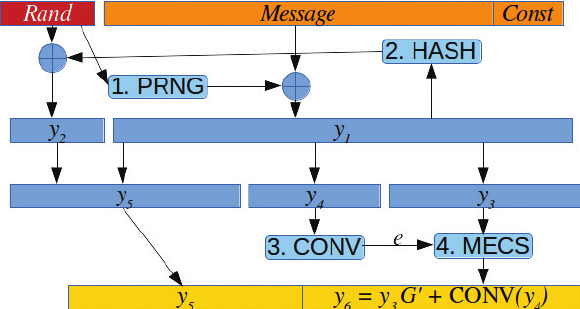
\includegraphics[width=0.7\textwidth]{materialy/kobara-imai-cca2.png}
    \caption{Diagram CCA2-odolné konverze \emph{Kobara-Imai}
    $\gamma$~\cite{Repka,Kobara}}
    \label{obr_cca2}
\end{figure}

%todo
\clearpage

% --------------------------------------------------------------------
\subsection{Odolnost vůči kvantovým počítačům}

Jeden z~hlavních důvodů popularity algoritmu \emph{McEliece} je fakt, není znám
algoritmus pro kvantový počítač, který by dokázal kryptosystém prolomit
rychleji, než na běžných počítačích~\cite{Dinh}. Kryptosystém je tak zařazen
mezi kandidáty asymetrické kryptografie pro tzv. \emph{post-kvantovou}
dobu~\cite{Post-Quantum_Cryptography} a~jeho varianta s~kvazi-cyklickými
\emph{MDPC} kódy se vyskytla v~draftu z~roku 2016 společnosti \emph{IEEE} mezi
doporučenými \emph{post-kvantovými} asymetrickými kryptosystémy~\cite{Schanck}.





% ====================================================================
% ====================================================================
% ====================================================================
\chapter{Implementace}\label{kap_implementace}

Pro implementaci kryptosystému \emph{McEliece} v~této práci jsme zvolili software
\emph{Wolfram Mathematica} \cite{Mathematica}. Tento software jsme zvolili hlavně
díky pohodlnosti některých matematických výpočtů a~konstrukcí a~také pro
přehlednost výstupů. %TODO

Při implementaci \emph{kryptosystému} se ukázaly nedostatky softwaru
\emph{Mathematica} a~bylo nutné zpracovat problematiku (rozšířených)
\emph{konečných těles} a~\emph{binárních Goppa kódů}. Tyto dvě oblasti byly
implementovány přímo v~softwaru \emph{Mathematica} tak, aby bylo možné jejich
pohodlné použití i v~jiných oblastech.

Celkově byla práce rozdělena do třech ucelených částí -- (binární) \emph{konečná
tělesa}, (ireducibilní) \emph{binární Goppa kódy} a~\emph{kryptosystém McEliece}
--, kde každou z~nich lze využít jako \emph{balík} či \emph{knihovnu} pro další
výpočty. V~následujících sekcích popíšeme jednotlivé části implementace, včetně
použitých algoritmů a~příkladů výpočtů. Příklady použití a~zdrojové kódy
implementace jsou k~nalezení na přiloženém disku a~též online
na~\url{https://github.com/VojtechMyslivec/mceliece-mathematica}.



% ====================================================================
\section{Binární konečná tělesa}\label{kap_implementace_teles}

V~této podkapitole pojednáváme o~implementaci \emph{binárních konečných těles}
včetně jejich \emph{rozšíření}. Zmíníme existující řešení v~softwaru
\emph{Mathematica}, zvolenou implementace a~popíšeme implementované algoritmy.

% --------------------------------------------------------------------
\subsection{Existující řešení}

Pro operace s~\emph{konečnými tělesy} v~softwaru \emph{Mathematica} byly
prostudovány interní funkce pro operace s~polynomy a~externí balík
\texttt{FiniteFields}. Vlastnosti těchto řešení popíšeme v~následujících
kapitolách.

\subsubsection{Operace s~polynomy}

Software \emph{Mathematica} obsahuje funkce pro operace s~polynomy nad reálnými
(případně i~komplexními) čísly. Většina těchto funkcí má volitelnou
\emph{možnost}\footnote{
    Anglicky se tento termín v~softwaru \emph{Mathematica} nazývá \emph{Option}.
} \emph{Modulus}, díky které lze zajistit, aby operace s~koeficienty byly
prováděny nad celými čísly \emph{modulo} zadané číslo $p$. Tímto způsobem je
možné implementovat operace nad tělesy $GF(p^n)$, nicméně je téměř nemožné tímto
způsobem implementovat \emph{rozšířená tělesa} -- polynomy nad polynomy.

Pro použití těchto funkcí (např. \texttt{ExtendedPolynomialGCD}, je třeba
polynomu v~úplném tvaru $\sum a_i x^i$ -- včetně $x^i$ s~tím, že $x$ musí být
nedefinovaný \emph{symbol}\footnote{
    Jinými slovy proměnná, která nemá definovanou hodnotu.
}. Tento požadavek je celkem nepraktický, protože definování této proměnné
kdekoliv v~programu by vedlo k~nemožnosti použití těchto funkcí. Navíc udržovat
si prvky ve formě např. $x^6 + x^3 + x + 1$ místo $1001011$ není pohodlné.
Další nevýhoda použití polynomů je, že software \emph{Mathematica} vypisuje
polynomy od \emph{nejnižšího} členu po \emph{nejvyšší} (např. $1+x^2+x^4+x^7$),
což je obrácený zápis, než je v~technické literatuře zvykem.


\subsubsection{Balík \texttt{FiniteFields}}

\paragraph{Balík} \emph{Balík} v~softwaru \emph{Mathematica} je soubor
obsahující rozšiřující funkce, které standardně nejsou k~dispozici. Balík je
možné načíst pomocí funkcí \texttt{Needs}, či případně \emph{Get}.

Balík \texttt{FiniteFields} obsahuje základní operace pro práci s~tělesy
$GF(p^n)$. Prvky konečných těles jsou pak určené \emph{seznamem}\footnote{
    \emph{Seznamem} se myslí struktura v~softwaru \emph{Mathematica}
    -- \emph{List}.
} koeficientů a~\emph{hlavičkou}, která určuje do jakého tělesa prvek patří.
Výhoda tohoto opatření je, že pro sčítání a~násobení je pak možné využít
obyčejné symboly operací ($+$,~$-$,~$*$,~$/$) a~operace se automaticky provede
v~daném tělese. Pro parametry $p$ a $n$ je určené jedno těleso $GF(p^n)$
(s~jedním konkrétním ireducibilním polynomem) a~\emph{seznam} koeficientů prvku
se opět píše od nejnižšího řádu po nejvyšší (například polynom $x^3 + x + 1$
z~tělesa $GF(2^5)$ je zapsán jako $GF[2,5][\{1,1,0,1,0\}] $).

Funkce z~balíku \texttt{FiniteFields} nejsou dostatečně zdokumentovány, jak je
jinak v~softwaru \emph{Mathematica} zvykem. Nepodařilo se využít funkcí z~tohoto
balíku pro operace s~\emph{rozšířenými tělesy}.


% --------------------------------------------------------------------
\subsection{Zvolené řešení}

Existující řešení pro práci s~\emph{konečnými tělesy} se ukázala jako
nedostačující. Jejich hlavní nevýhodou je nemožnost použití při výpočtech
s~\emph{rozšířenými tělesy}. Proto bylo implementováno vlastní řešení pro práci
s~\emph{konečnými tělesy}.

Při implementaci operací nad \emph{konečnými tělesy} bylo dodržováno následující
jednotné rozhraní:

\begin{itemize}
    \item Prvky \emph{konečných těles} reprezentujeme \emph{seznamem}
        koeficientů od nejvyššího po nejnižší. \\
        U~\emph{rozšířených těles} jsou koeficienty opět prvky konečných těles. \\
        Například polynom $x^3+x+1$ je reprezentován seznamem: $\{1,0,1,1\}$ \\
        a~polynom $(y+1)x^2 + (y)$ je reprezentován:
        $\left\{\{1,1\},\{0,0\},\{1,0\}\right\}$

    \item Prvek (seznam koeficientů) může být libovolně dlouhý. V~případě
        potřeby se při výpočtu \emph{redukuje} (ireducibilním) polynomem nebo
        dorovná \emph{nulovými} koeficienty.

    \item Počet koeficientů vnitřních prvků (koeficientů) musí být vždy stejný. \\
        Například prvek $\{\{0,0\},\{1\},\{1,0\}\}$ není platný.

    \item Jednotlivým funkcím je kromě operandů předáván též i~\emph{modul}
        skládající se z~odpovídajících (ireducibilních) polynomů, včetně
        charakteristiky tělesa. Tento \emph{modul} je definovaný následovně:
        \begin{itemize}
            \item Pro tělesa $GF(p^{n_1})$ je \emph{modul} složen
                z~(ireducibilního) polynomu $i_1$ stupně~$n_1$ a~dané
                charakteristiky $p$:\\
                $modul_1 = \left\{i_1,p\right\}$
            \item Pro rozšířená tělesa se \emph{modul} skládá z~odpovídajícího
                \emph{polynomu} $i_k$ stupně $n_k$ nad tělesem $GF(
                {{p^{n_1}})^{\ldots}}^{n_{k-1}}$ a~\emph{modulu vnitřního
                tělesa}: \\
                $modul_k = \left\{i_k,modul_{k-1}\right\}$.
        \end{itemize}

    \item Všem funkcím se předávají nejdřív \emph{operandy} a~poté
        \emph{modul}.\\
        Například pro prvky $a,b\in GF(p^{\ldots})$, $m\in\mathbb{N}$
        a~odpovídající $modul$: \\
        \hspace*{0.6cm}$krat[a,b,modul]$ \\
        \hspace*{0.6cm}$inverze[a,modul]$ \\
        \hspace*{0.6cm}$mocnina[a,e,modul]$ \\
        \hspace*{0.6cm}\ldots

    \item Pro implementaci operací v~tělesech $GF(p^n)$ jsou použité vnitřní
        funkce softwaru \emph{Mathematica} pro práci s~\emph{polynomy}.
        Implementované funkce pro tato tělesa tedy zpravidla obsahují převod ze
        \emph{seznamu} čísel na \emph{polynom}, zavolání vnitřní funkce pro
        \emph{polynomy} a~převodu zpět na \emph{seznam} koeficientů. Díky těmto
        vnitřním funkcím je docíleno rychlejšího výpočtu, než kdyby byla použita
        vlastní implementace nad \emph{seznamy} celých čísel.

    \item Pro implementaci operací v~\emph{rozšířených tělesech} byly
        implementovány jednotlivé algoritmy operací (popsané níže), jelikož
        nebylo možné použít pro tyto operace vnitřní funkce softwaru
        \emph{Mathematica}. Funkce nad \emph{rozšířenými tělesy} zpravidla
        volají odpovídající funkce ve vnitřních tělesech (například násobení
        jednotlivých \emph{koeficientů}).

\end{itemize}

Tato pravidla umožňují pohodlný, jednotný a \emph{rekurzivní} přístup
k~jednotlivým prvkům a voláním funkcí (druhá složka \emph{modulu} je
\emph{modul} \emph{vnitřního tělesa}, prvky \emph{polynomu} jsou opět
\emph{polynomy}, \ldots).

\paragraph{Poznámka:} Ač jsou funkce implementované v~co nejobecnějším pojetí,
tak je kladen důraz na efektivnost výpočtů vzhledem k~\emph{binárním} tělesům --
tedy k~\emph{tělesům} s~charakteristikou $2$. Pro \emph{tělesa} s~jinou
charakteristikou není chování funkcí definováno.

% --------------------------------------------------------------------
\subsection{Implementace operací}

V~následujících kapitolách je popsána implementace hlavních operací
v~\emph{konečných tělesech} a použitých algoritmů. Pro další informace je
doporučeno nahlédnout do zdrojového kódu a~příkladů použití.

V~níže uvedených pseudokódech se používá některých prvků ze syntaxe softwaru
\emph{Mathematica}:

\begin{table}[!ht]
    \centering
    \begin{tabular}{l  l}
        Zápis               & Význam                                            \\
        \hline
        \texttt{foo[bar]}   & Volání funkce \emph{foo} s~argumentem \emph{bar}  \\
        \texttt{ham[[i]]}   & \emph{i}-tý prvek seznamu (pole) \emph{ham}       \\
    \end{tabular}
    \caption{Prvky syntaxe jazyka softwaru \emph{Mathematica}}
\end{table}


\subsubsection{Sčítání}

Jelikož operace sčítání se v~jakémkoliv \emph{tělese} provádí po jednotlivých
koeficientech \emph{modulo} $p$, je tato funkce jediná volána místo celkového
modulu pouze se zadanou charakteristikou $p$.

Pro \emph{rozšířená tělesa} funkce rekurzivně volá stejnou operaci sčítání na
jednotlivé koeficienty zadaných polynomů až na úroveň obyčejných jednorozměrných
seznamů. Pro sčítání těchto prvků funkce používá obyčejné sčítání dvou seznamů
modulo $p$.

\begin{algoritmus}[!ht]
    \caption{Sčítání prvků}
    \begin{algorithmic}[1]
     \Function{plus[ $a$, $b$, $p$ ]}{}\Comment{Pro $GF(p^n)$, $p$ je prvočíslo}
        \State \Return $Mod[a+b,p]$
     \EndFunction
    \end{algorithmic}
    \begin{algorithmic}[1]
     \Function{plus[ $a$, $b$, $p$ ]}{}\Comment{Pro $GF(q^n)$, $q$ je $p^{\ldots}$}
        \For{$ i \gets 1\ldots Length[a] $}
            \State $c[[i]] \gets plus[a[[i]],b[[i]],p]$
        \EndFor
        \State \Return $c$
     \EndFunction
    \end{algorithmic}
\end{algoritmus}

\paragraph{Poznámka:} U~dalších operací s~prvky z~tělesa $GF(p^n)$ (kde $p$ je
prvočíslo) se prvky (\emph{seznamy}) převádějí na polynomy a~využívá se
implementovaných funkcí softwaru \emph{Mathematica}. Z~tohoto důvodu jsou nadále
uváděné algoritmy pouze pro \emph{rozšířená tělesa} $GF(q^n)$, kde $q$ je nějaká
mocnina prvočísla.


\subsubsection{Redukce polynomu}

Redukce polynomu (neboli \emph{modulo} polynom) se používá ve většině dalších
funkcí. Tato funkce se volá se dvěma parametry -- prvkem $a$ a~polynomem
(\emph{modulem}) $m$. Funkce vrátí zbytek polynomu $a$ po dělení polynomem $m$.

Redukce polynomu pro \emph{rozšířená tělesa} je inspirovaná \emph{Comb metodou}
z~\cite{Merchan}. K~původnímu prvku $a$ se opakovaně přičítá (od nejvyššího
řádu) patřičný násobek \emph{polynomu} $m$ tak, aby se daný koeficient $a_i$
rovnal nule (viz příklad níže).

Pro $GF(p^n)$ se používá interní funkce \texttt{PolynomialMod}

\begin{algoritmus}[!ht]
    \caption{Redukce prvku v~tělese s~charakteristikou $2$}
    \begin{algorithmic}[1]
     \Function{redukuj[ $a$, $\left\{m, modul_{vnitrni}\right\}$ ]}{}
        \State $ l_a \gets stupen[a] + 1 $
            \Comment{Délka redukovaného polynomu}
        \State $ l_m \gets stupen[m]$
            \Comment{Výsledná délka redukovaného polynomu}

        // Převedení $m$ na \emph{monický} polynom
        \State $ koef \gets inverze[ m[[1]], modul_{vnitrni} ] $
            \Comment{Inverze nejvyššího koeficientu}
        \State $ m \gets krat[ koef, m, modul_{vnitrni} ] $
            \Comment{Násobení skalárem}

        \hfil
        \State $ m \gets PadRight[ m, l_a - l_m ] $
            \Comment{Natáhnutí polynomu na délku $a$}

        \For{$ i \gets 1 \ldots l_a - l_m $}
            \State $ s \gets krat[ a[[i]], m, modul_{vnitrni} ] $
                \Comment{Skalární násobek}
            \State $ a \gets plus[ a, s, 2 ] $
                \Comment{Odečtení v~binárním tělese}
            \State $ m \gets RotateRight[m] $
                \Comment{Posunutí redukovaného polynomu}
        \EndFor

        \hfil
        \State \Return $a$

     \EndFunction
    \end{algorithmic}
\end{algoritmus}

\paragraph{Příklad} Redukce polynomu $(10)x^5 + (10)x^4 + (01)$
polynomem $(10)x^3 + (01)x^2 + (11)x + (10)$ (nad tělesem $GF(2^2)$
s~ireducibilním polynomem $111$):

\renewcommand{\0}{{\textcolor[gray]{0.75}{(00)}}}
\begin{align*}
&(10)(10)(00)(00)(00)(01) \mod (10)(01)(11)(10) : \\
& \arraycolsep=1pt
\begin{array}{*{6}{l}}
        (10) & (10) & (00) & (00) & (00) & (01) \\
    \hline
        (10) & (01) & (11) & (10) &  \0  &  \0  \\
         \0  & (11) & (10) & (01) & (11) &  \0  \\
         \0  &  \0  & (01) & (11) & (10) & (01) \\
    \hline
             &      &      & (00) & (01) & (00) \\
\end{array}
\end{align*}

$
    \Rightarrow
    \left| (10)(10)(00)(00)(00)(01) \right|_{(10)(01)(11)(10)} = (00)(01)(00)
$


\subsubsection{Násobení}

Výsledkem násobení dvou polynomů $a$ a~$b$ stupně $n$ a~$m$ je polynom $c$
stupně $n+m$. Násobení je implementováno tak, že k~výsledku $c$ (na počátku je
to nulový polynom) se postupně přičítá skalární násobek polynomu $b$ koeficienty
polynomu $a$, který je zároveň \emph{posunutý} o~patřičný počet pozic. Využívá
se zde faktu, že násobení libovolného \emph{polynomu} $A(x)$ a~$x^i$ je posunutí
koeficientů polynomu $A$ o~$i$ pozic doleva. Výsledný polynom $c$ je následně
\emph{redukován} zadaným modulem (viz výše).

Pro $GF(p^n)$ se používá obyčejného násobení dvou \emph{polynomů} a~následné
\emph{redukce} \emph{modulem}.

\begin{algoritmus}[!ht]
    \caption{Násobení prvků}
    \begin{algorithmic}[1]
     \Function{krat[ $a$, $b$, $\left\{m, modul_{vnitrni}\right\}$ ]}{}
        \State $ p \gets charakteristika[ modul ] $
            \Comment{Charakteristika tělesa}

        // Natažení na výslednou délku
        \State $ b \gets PadLeft[ b, stupen[a] + stupen[b] + 1 ] $
        \State $ c \gets nulovyPolynom[\ldots ] $
            \Comment{Nulový polynom nad vnitřním tělesem}

        \hfil
        \For{$ i \gets stupen \ldots 1 $}
            \State $ s \gets krat[ a[[i]], b, modul_{vnitrni} ] $
                \Comment{Skalární násobek}
            \State $ c \gets plus[ c, s, p ] $
            \State $ b \gets RotateLeft[b] $
                \Comment{Posunutí přičítaného polynomu}
        \EndFor

        \hfil
        \State \Return $redukuj[c,modul]$
     \EndFunction
    \end{algorithmic}
\end{algoritmus}

\paragraph{Příklad} Násobení polynomu $(110)x^2 + (101)x + (001)$ polynomem
$(001)x^3 + (010)x + (011))$ (nad tělesem $GF(2^3)$ s~ireducibilním
polynomem $1011$):

\renewcommand{\0}{{\textcolor[gray]{0.75}{(000)}}}
\begin{align*}
& (110)(101)(001) \cdot (001)(000)(010)(011) : \\
& \arraycolsep=1pt
\begin{array}{r *{8}{l}}
        (001) x^3 : \quad \; & (110) & (101) & (001) &   \0  &   \0  &   \0  \\
        (000) x^2 : \quad \; &   \0  & (000) & (000) & (000) &   \0  &   \0  \\
        (010) x^1 : \quad \; &   \0  &   \0  & (111) & (001) & (010) &   \0  \\
        (011) x^0 : \quad \; &   \0  &   \0  &   \0  & (001) & (100) & (011) \\
    \hline
                             & (110) & (101) & (110) & (000) & (110) & (011) \\
\end{array}
\end{align*}

$\Rightarrow$ Výsledek operace násobení modulo polynom $g$ se získá redukcí
polynomu $(110)(101)(110)(000)(110)(011)$ polynomem $g$.


\subsubsection{Inverze}\label{kap_implementace_inverze}

Výpočet multiplikativní \emph{inverze} je implementován pomocí \emph{rozšířeného
Euklidova algoritmu}. Tento algoritmus se často vizualizuje jako výpočet tabulky
po řádkách (viz níže). Ve skutečnosti však pro výpočet dalšího řádku stačí
pracovat s~hodnotami dvou řádků předešlých. Proto si není nutné udržovat
v~paměti celou tabulku, ale stačí si udržovat hodnoty dvou řádků a~po výpočtu
třetího hodnoty posunout.

Výpočet hodnot dalšího řádku tabulky probíhá následovně:

\begin{itemize}
    \item Hodnoty předchozích řádků jsou:\\
        \hspace*{0.6cm}Polynomy $p_{i-2}$ a $p_{i-1}$ (na začátku inicializovány
            na ireducibilní polynom $m$ a \emph{prvek}, ke kterému je hledaná
            inverze). \\
        \hspace*{0.6cm}Polynomy $k_{i-2}$ a $k_{i-1}$ (na začátku inicializovány
            na $0$ a~$1$, respektive \emph{nulový} a~\emph{jednotkový
            polynom}).

    \item Je spočítán \emph{podíl} $q$ a~zbytek $p_i$ pomocí tzv. \emph{dlouhého
        dělení} polynomu $p_{i-2}$ polynomem $p_{i-1}$.

    \item Je spočítán \emph{polynom} $k_i = k_{i-2} - q \cdot k_{i-1} $

    \item Tyto kroky se opakují, dokud není získán polynom $p_i$ stupně $0$
        (jinými slovy jediný prvek vnitřního tělesa).

    \item Výsledná \emph{inverze} se získá jako skalární násobek \emph{polynomu}
        $k_i$ inverzí (posledního) \emph{koeficientu} polynomu $p_i$.
\end{itemize}

Inverze v~$GF(p^n)$ je implementovaná pomocí interní funkce
\texttt{Polynomial\-ExtendedGCD}.

\paragraph{Poznámka:} Pro výpočet dělení je v~\emph{rozšířených tělesech}
potřeba vypočítat inverzi největšího koeficientu dělitele\footnote{
    Zde je patrná rekurzivní vlastnost tohoto algoritmu, kdy pro výpočet inverze
    prvku v~tělese $GF(q^n)$ je třeba vypočítat inverzi v~tělese $GF(q)$.
} a~dále je algoritmus realizován posouváním dělitele a~následnou redukcí pomocí
sčítání.

\begin{algoritmus}[!ht]
    \caption{Inverze prvků -- \emph{Rozšířený Euklidův algoritmus}}
    \begin{algorithmic}[1]
     \Function{inverze[ $prvek$, $modul:\left\{ m, modul_{vnitrni} \right\}$ ]}{}
        \State $ A \gets m $; $ B \gets prvek $

        // Inicializace na \emph{jednotkový} resp. \emph{nulový} polynom z~tělesa
        \State $ k_A \gets nulovyPolynom[\ldots] $;
            $ k_B \gets jednotkovyPolynom[\ldots] $
        \While{$stupen[B] \neq 0 $}

            // Výpočet $q$ a $C$ pomocí dlouhého dělení v~jednom kroku
            \State $ q   \gets A/B $; $ C   \gets A \mod B $
            \State $ k_C \gets k_A - krat[ q, k_B, modul ] $
            \State $ A \gets B$; $k_A \gets k_B$
            \State $ B \gets C$; $k_B \gets k_C$
        \EndWhile

        // Výpočet koeficientu ve vnitřním tělese
        \State $koef \gets inverze[ Last[C], modul_{vnitrni} ]$
        \State \Return $krat[ koef, k_C, modul_{vnitrni} ]$\Comment{Násobení skalárem}
     \EndFunction
    \end{algorithmic}
    \label{alg_eea}
\end{algoritmus}

\paragraph{Příklad} \emph{Rozšířený Euklidův algoritmus} pro výpočet
\emph{inverze} polynomu \\
$(101)x^3 + (010)x^2 + (110)x + (111)$ \emph{modulo} $(001)x^4 + (011)x^3 +
(011)x^2 + (001)x + (011)$ (nad tělesem $GF(2^3)$ s~ireducibilním polynomem
$1101$):

\begin{center}
    \begin{tabular}{r|r r}
               Podíl &                      Zbytek &            Koeficienty \\
            \hline
            \hline
                     & $(001)(011)(011)(001)(011)$ & $               (000)$ \\
                     & $     (101)(010)(110)(111)$ & $               (001)$ \\
            \hline
        $(111)(000)$ & $          (110)(011)(011)$ & $          (111)(000)$ \\
        $(111)(001)$ & $               (001)(100)$ & $     (010)(111)(001)$ \\
        $(110)(001)$ & $                    (111)$ & $(001)(111)(110)(001)$ \\
    \end{tabular}
\end{center}

$
    \Rightarrow
    \left|(101)(010)(110)(111)^{-1}\right|_{(001)(011)(011)(001)(011)} =
    (101)(001)(100)(101)
$


\subsubsection{Druhá mocnina}\label{kap_druha_mocnina}

Pro prvky tělesa s~\emph{charakteristikou} $2$ je výhodné implementovat funkci
\uv{na druhou} díky následujícímu tvrzení:

\begin{tvrzeni}
    Nechť $A=(a_n \ldots a_2 a_1 a_0)$ je prvek tělesa s~\emph{charakteristikou}
    $2$, potom platí:
    $$ A^2 = (a_n^2 0 \ldots 0 a_2^2 0 a_1^2 0 a_0^2) $$
\end{tvrzeni}

S~využitím tohoto tvrzení je realizace funkce na počítání druhé mocniny
triviální:

\begin{itemize}
    \item Provedení druhé mocniny všech koeficientů.
    \item Proložení koeficientů polynomu nulovými koeficienty.
    \item Redukování polynomem (viz výše).
\end{itemize}

%todo
\vfil

\begin{algoritmus}[!ht]
    \caption{Umocňování na druhou v~tělese s~charakteristikou $2$}
    \begin{algorithmic}[1]
     \Function{naDruhou[ $a$, $\left\{m, modul_{vnitrni}\right\}$ ]}{}
        \For{$ i \gets 1 \ldots Length[i]$}
            \State $ a[[i]] \gets naDruhou[ a[[i]], modul_{vnitrni} ] $
        \EndFor
        \State $ nula \gets nulovyPolynom[ \ldots ]$
            \Comment{Odpovídající nulový koeficient}
        \State $ a \gets Riffle[ a, nula ] $
            \Comment{Proloží koeficienty prvkem $nula$}
        \State \Return $ redukujPolynom[ a, modul ] $
     \EndFunction
    \end{algorithmic}
\end{algoritmus}

%TODO poradi
\paragraph{Náznak důkazu}
\begin{align*}
    A(x)     &=  a_n x^n + \ldots + a_2 x^2 + a_1 x + a_0 \\
    {A(x)}^2 &=  (a_n x^n + \ldots + a_2 x^2 + a_1 x + a_0)\cdot(a_n x^n + \ldots + a_2 x^2 + a_1 x + a_0) = \\
             &= a_n x^n   \cdot (a_n x^n + \ldots + a_2 x^2 + a_1 x + a_0) + {}                              \\
             & \qquad \vdots                                                                                 \\
             &  {} + a_2 x^2   \cdot (a_n x^n + \ldots + a_2 x^2 + a_1 x + a_0) + {}                         \\
             &  {} + a_1 x \, \:  \cdot (a_n x^n + \ldots + a_2 x^2 + a_1 x + a_0) + {}                      \\
             &  {} + a_0 \quad \cdot (a_n x^n + \ldots + a_2 x^2 + a_1 x + a_0) =                            \\
             &= a_n^2 x^{2n}    + \ldots + a_n a_2 x^{n+2} + a_n a_1 x^{n+1} + a_n a_0 x^n + {}              \\
             & \qquad \vdots                                                                                 \\
             &  {} + a_n a_2 x^{n+2} + \ldots + a_2^2 x^4       + a_2 a_1 x^3     + a_2 a_0 x^2 + {}         \\
             &  {} + a_n a_1 x^{n+1} + \ldots + a_2 a_1 x^3     + a_1^2 x^2       + a_1 a_0 x   + {}         \\
             &  {} + a_n a_0 x^n     + \ldots + a_2 a_0 x^2     + a_1 a_0 x       + a_0^2       =            \\
             &= a_n^2 x^{2n} + \ldots  + 2 ( a_3 a_0 + a_2 a_1 ) x^3  + 2 ( a_2 a_0 ) x^2 + a_1^2 x^2 + 2 ( a_1 a_0 ) x + a_0^2 = \\
             &= \sum_{i=0}^{n} a_i^2 x^{2i} + 2 \sum_{i=1}^{n+1}\sum_{\substack{j<k \\ j+k = i}} a_j a_k =   \\
             &= \sum_{i=0}^{n} a_i^2 x^{2i}
    \hspace{2.5cm} \cong (a_n^2 0 \ldots 0 a_2^2 0 a_1^2 0 a_0^2)
\end{align*}


\subsubsection{Mocnění}

Mocnění \emph{polynomů} je implementováno pomocí algoritmu
\emph{Square-and-Multiply} (\emph{SM}). Algoritmus využívá faktu, že libovolnou
mocninu lze rozložit na součin mocnin čtverců ($^2$, $^4$, $^8$, \ldots). Konkrétně
byla implementována varianta provádějící výpočet od nejvíce významného bitu
exponentu\footnote{
    Uváděna jako \emph{MSB} -- z~anglického \emph{Most Significant Bit}.
}. Algoritmus má vstupy polynom $a$ a~exponent $e$. Exponent se vyjádří jako
číslo v~\emph{binární} soustavě a~poté algoritmus provádí cyklus přes bity
tohoto rozvoje. V~každém kroku se mezivýsledek umocní na druhou a~v~případě, že
je odpovídající bit exponentu $1$, přinásobí se původní číslo $a$.


\begin{algoritmus}[!ht]
    \caption{Umocňování prvku $a^e \mod modul$ -- \emph{Square-and-Multiply}}
    \begin{algorithmic}[1]
     \Function{umocni[ $a$, $e$, $modul$ ]}{}
        \If{$ e = 0 $}
            \State \Return $nulovyPolynom[\ldots]$
                \Comment{Nulový prvek tělesa}
        \EndIf
        \State $ rozvoj \gets IntegerDigits[ e, 2 ] $
            \Comment{Binární rozvoj exponentu}
        \State $ c \gets a $
            \Comment{$rozvoj[[1]]$ je vždy $1$}
        \For{$ i \gets 2 \ldots Length[rozvoj] $}
            \State $ s \gets naDruhou[ c, modul ] $
            \State $ m \gets krat[ s, a, modul ] $
            \If{$ rozvoj[[i]] = 0 $}
                \State $ c \gets s $
            \Else
                \State $ c \gets m $
            \EndIf
        \EndFor
        \State \Return $c$
     \EndFunction
    \end{algorithmic}
\end{algoritmus}


\paragraph{Poznámka:} Takto implementovaný algoritmus je zranitelný vůči
odběrové a~časové analýze. Pro odolnou implementaci je nutné počítat násobek
\emph{vždy} a~pokud je daný bit exponentu $1$, přiřadit násobek do mezi výpočtu.
Pseudokód i~reálná implementace je prováděna tímto (bezpečným) způsobem.

\paragraph{Příklad} Algoritmus \emph{Square-and-Multiply} pro výpočet
$\left( (11)x^2 + (10) \right)^{26}$ \emph{modulo} $(01)x^3 + (11)x + (01)$
(nad tělesem $GF(2^2)$ s~ireducibilním polynomem~$111$):

\renewcommand{\0}{{\textcolor[gray]{0.75}{(00)}}}
\begin{center}
    \begin{tabular}{c|r|l|r|r}
        \multirow{2}{*}{Op.} & \multicolumn{2}{c}{Mocnina} & \multicolumn{1}{c}{\multirow{2}{*}{Výpočet}} & \multirow{2}{*}{Výsledek} \\
                &  dek. & bin.    &                                     &                \\
        \hline
        \hline
                & $  1$ & $1    $ &                                     & $(11)(00)(10)$ \\
        \hline
    \textbf{S}  & $  2$ & $1    $ & $                (10)\0(00)\0(11) $ & $(01)(10)(11)$ \\
    \textbf{M}  & $  3$ & $11   $ & $ (01)(10)(11) \cdot (11)(00)(10) $ & $(10)(11)(00)$ \\
        \hline
    \textbf{S}  & $  6$ & $110  $ & $                (11)\0(10)\0(00) $ & $    (11)(00)$ \\
        \hline
    \textbf{S}  & $ 12$ & $1100 $ & $                      (10)\0(00) $ & $(10)(00)(00)$ \\
    \textbf{M}  & $ 13$ & $1101 $ & $ (10)(00)(00) \cdot (11)(01)(10) $ & $    (01)(00)$ \\
        \hline
    \textbf{S}  & $ 26$ & $11010$ & $                      (01)\0(00) $ & $(01)(00)(00)$ \\
    \end{tabular}
\end{center}
$
    \Rightarrow
    \left| (11)(00)(10)^{26} \right|_{(01)(00)(11)(01)} = (01)(00)(00)
$

% --------------------------------------------------------------------
\subsection{Možná zlepšení}

V~této kapitole nastíníme možná zlepšení implementace, která zrychlují
výpočet některých operací.


\subsubsection{Logaritmické tabulky}

Pro zrychlení výpočtu násobení a~mocnin prvku lze v~\emph{konečném tělese}
využít faktu, že vždy existuje \emph{primitivní prvek} a~převádět tak operace
v~tělese na operace s~celými čísly.

\begin{definice}
    Nechť $\alpha$ je \emph{generátor} \emph{multiplikativní grupy} tělesa
    $\mathbb{F}$. Potom říkáme, že $\alpha$ je \emph{primitivní prvek} tělesa
    $\mathbb{F}$.
\end{definice}

\paragraph{Důsledek} Každý prvek tělesa $\mathbb{F}$ -- kromě \emph{nulového}
prvku \emph{aditivní grupy} -- lze vyjádřit jako $\alpha^i$ pro nějaké $i$.

Důkaz plyne přímo z~definice.

Násobení dvou prvků $a = \alpha^{i_a}$ a~$b = \alpha^{i_b}$ tak můžeme převést
na součet mocnin \emph{primitivního prvku}:
$$ a \cdot b = \alpha^{i_a} \cdot \alpha^{i_b} = \alpha^{i_a + i_b} $$

Podobným způsobem můžeme zjednodušit umocňování prvku:
$$ a^e = \left(\alpha^i\right)^e = \alpha^{i e} $$

V~obou případech je samozřejmě možné použít \emph{Eulerovu větu} a~mocniny
redukovat \emph{modulo} $N$, kde $N$ je počet prvků \emph{multiplikativní grupy
tělesa} ($N=p^n-1$ pro těleso $GF(p^n)$). Jakoukoliv operací násobení a~mocnění
získáme prvek $\alpha^{n_c}$, kde $n_c$ je celé číslo v~rozsahu od $0$ do $N-1$.

Reprezentací prvků pomocí odpovídajících mocnin \emph{primitivního prvku} se tak
můžeme vyhnout násobení a~umocňování prvků v~tělese a~nahradit ho sčítáním
a~násobením celých čísel, což je řádově jednodušší. V~případě sčítání prvků
v~tělese je však nutné mít jejich standardní reprezentaci (seznam koeficientů),
jelikož se sčítání provádí po jednotlivých koeficientech, respektive bitech.
Není možné nahradit sčítání dvou prvků jiné operaci s~mocninami
\emph{primitivního prvku}.

Pro použití tohoto zrychlení výpočtů je tak nutné připravit v~paměti programu
překladové \emph{log}- a~\emph{antilogaritmické} tabulky pro překlad prvků
z~jedné reprezentace na druhou.

% todo
\clearpage

Ač se tak získá podstatné zrychlení výpočtů v~tělese, existuje několik nevýhod
tohoto přístupu:

\begin{itemize}
    \item Je nutné nalézt \emph{primitivní prvek tělesa}.

    \item Je nutné vygenerovat a uchovat v~paměti počítače obě tabulky pro
        překlad.
        \begin{itemize}
            \item Tato tabulka lze implementovat pomocí obyčejného pole či
                sezna\-mu, kde se k~danému indexu v~seznamu vyskytuje
                odpovídající hodnota.
            \item Pro binární  tělesa $GF(2^m)$ je velikost jedné tabulky
                $O(m 2^m)$ (konkrétně $2^m - 1$ hodnot, kde každá je
                reprezentována $m$ bity).
            \item Jelikož je paměťová náročnost \emph{exponenciální}, můžeme
                tyto tabulky uchovávat pouze pro \emph{malá} $m$ (např. $8$ či
                $16$, nikoliv však $1024$).
        \end{itemize}

    \item \emph{Nulový prvek} tělesa není možné žádným způsobem zobrazit jako
        mocninu. Při každé operaci je potřeba s~touto skutečností počítat
        a~hlídat jako výjimku.

\end{itemize}

Toto vylepšení bychom mohli využít pro operace ve \emph{vnitřním tělese}
$GF(2^m)$, nad kterým jsou postavené polynomy v~\emph{binárních Goppa kódech}.


\subsubsection{Implementace dělení}

Dělení prvkem $b$ v~\emph{konečném tělese} převádíme na násobení $b^{-1}$. Pro
výpočet \emph{podílu} se tak počítá inverze a~následně násobek. Je ale možné
implementovat rovnou algoritmus pro dělení.

Algoritmus pro dělení prvku $a$ prvkem $b$ je totožný s~algoritmem pro výpočet
\emph{inverze} prvku $b$ s~tím rozdílem, že je počáteční hodnota koeficientu
$k_b$ (viz \emph{EEA} -- alg. \ref{alg_eea}) nastavena na hodnotu $a$.
%Jelikož průběh algoritmu odpovídá ekvivalentním úpravám rovnic, algoritmus
%skončí s rovnicí:
%
%$$ 1 = (l \cdot a ) \cdot b  + k \cdot m $$
Výsledkem algoritmu pak bude inverze prvku $b$ vynásobená $a$, což přesně
odpovídá výrazu $a/b$.

% todo pozice
\clearpage

% ====================================================================
\section{Ireducibilní binární Goppa kódy}

Pro implementaci kryptosystému jsme zvolili \emph{ireducibilní Goppa kódy},
které jsme popsali v~kapitole~\ref{kap_goppa_kody}.
V~podkapitole~\ref{kap_generovani} popíšeme algoritmy, které slouží pro
vygenerování kódu dle zadaných parametrů a~v~podkapitole~\ref{kap_patterson}
\emph{Pattersonův} algoritmus pro dekódování a~(opravu) chyb vzniklých při
přenosu.


% --------------------------------------------------------------------
\subsection{Generování Goppa kódu}\label{kap_generovani}

Parametry \emph{ireducibilního binárního Goppa kódu} $(n,k,t)$ jsou jednoznačně
určené parametry~$m$ a~$t$. Parametr~$m$ určuje řád vnitřního tělesa $GF(2^m)$
a~parametr~$t$ stupeň (ireducibilního) \emph{Goppova} polynomu~$g$. Parametr~$n$
(počet prvků podpory~$L$) je $2^m$, protože posloupnost~$L$ obsahuje
\emph{všechny} prvky z~tělesa $GF(2^m)$. Redundance takového kódu je $r=mt$,
jelikož vygenerovaná matice~$H$ má $t$~řádků nad tělesem $GF(2^m)$, neboli
$mt$~řádků nad tělesem $GF(2)$. Parametr~$k$ je pak jednoznačně určený
z~definice kódu jako $n-k$ tedy $2^m-mt$.

Pro sestrojení \emph{kontrolní} matice~$H$ potřebujeme vygenerovat
\emph{podporu} kódu~$L$ a~matice $V$ a~$D$. Pro sestrojení těchto objektů je též
třeba vygenerovat \emph{modul} vnitřního tělesa~$GF(2^m)$ a~samozřejmě
\emph{Goppův} polynom $g$. Pro sestrojení \emph{modulu} využijeme funkcí
definovaných v~předešlé kapitole~\ref{kap_implementace_teles} a~pro vygenerování
matic a~podpory jsou implementovány dílčí funkce popsané níže.

\begin{algoritmus}[!ht]
    \caption{Generování Goppa kódu}
    \begin{algorithmic}[1]
     \Function{generujGoppaKod[ $m$, $t$ ]}{}
        \State $ n \gets 2^m ; \quad r \gets t m ; \quad k \gets n - r $

        // ireducibilní \emph{Goppův} polynom $g$ stupně $t$ nad tělesem $GF(2^m)$
        \State $ modul \gets generujModul[ \{ 2, m \}, t ] $
        \State $ \{ g, modul_{vnitrni} \} \gets modul $

        \hfil
        \State $ L \gets generujPodporuL[ m ] $
            \Comment{Generování posloupnosti $L$}
        \State $ V \gets maticeV[ podporaL, t, modul_{vnitrni} ] $
            \Comment{\emph{Vandermondova} matice}
        \State $ D \gets maticeD[ podporaL, modul ] $
            \Comment{\emph{Diagonální} matice}

        \hfil
        \State $ H \gets dotNadF[ V, D, modul_{vnitrni} ] $
            \Comment{Násobení matic nad $GF(2^m)$}
        \State $ H \gets Flatten[Transpose \mathbin{/@} H, 1 ] $
            \Comment{\emph{Rozbalení} prvků matice $H$}

        // Převod matice $H$ na $G$ -- \emph{ortogonální doplněk}
        \State $ G \gets NullSpace[ H, Modulus \to 2 ] $

        \hfil
        \State $ X \gets \{ jednotkovyPolynom[\ldots], nulovyPolynom[\ldots] \} $
            \Comment{Polynom~$x$}

        // předpočítané dílčí syndromy $\left(x-L_i\right)^{-1}$
        \For{$ i \gets 1 \ldots n $}
            \Comment{Ve skutečnosti pomocí funkce \texttt{Map}}
            \State $ syndromyL[[i]] \gets inverze[ plus[X, L[[i]], 2], modul ] $
        \EndFor

        \hfil
        \State \Return $ \{ G, modul, L, syndromyL \}$
     \EndFunction
    \end{algorithmic}
\end{algoritmus}


\paragraph{Generování \emph{Goppova} polynomu} \hfil \\
Pro sestrojení \emph{ireducibilního Goppa kódu} je potřeba vygenerovat
\emph{ireducibilní} polynom nad konečným tělesem $GF(2^m)$. Pro skutečné
generování náhodného ireducibilního polynomu by bylo třeba implementovat test
ireducibility polynomu (např. dle~\cite{Gao}). Pro použití \emph{Goppa} kódů
v~této práci bylo několik ireducibilních polynomů předgenerováno v~softwaru
\emph{SageMath}~\cite{Sage}.


\paragraph{Podpora $L$} \hfil \\
Generování podpory~$L$ je velmi jednoduché. Dle parametru~$m$ se vygenerují
všechny vektory z~$\{0,1\}^m$ a~náhodně se permutují (zamíchají). Tuto funkci
lze jednoduše řešit pomocí vnitřních funkcí softwaru \emph{Mathematica}
\texttt{Tuple} a~\texttt{Ran\-domSample}. % todo rozdeleni slov


\paragraph{Matice $D$} \hfil \\
Matice~$D$ je diagonální $n \times n$ maticí (nad $GF(2^m)$), kde na diagonále
jsou inverze v~$GF(2^m)$ prvků~z~$L$ dosazených do polynomu $g$, neboli $D_{i,i}
= g(L_i)^{-1}$. Pro výpočet této matice je potřeba zadat \emph{modul} tělesa
$GF(2^m)$, polynom~$g$ a~podporu~$L$. Výpočet je pak proveden pomocí
\emph{aplikování} (\texttt{Map}) funkcí dosazení do polynomu a~inverze
v~tělese na prvky seznamu $L$.\footnote{
    Zde by šlo dosazení do polynomu všech prvků z~$L$ zrychlit stejným způsobem,
    jako byl uvedený u~\emph{Chienova} hledání kořenů
    v~kapitole~\ref{kap_goppa_dekodovani}.
}


\paragraph{Matice $V$} \hfil \\
\emph{Vandermondova} $n \times t$ matice~$V$ nad $GF(2^m)$ obsahuje na prvním
řádku \emph{jednotkové prvky} a~na dalších řádcích mocniny prvků z~$L$.
Konkrétně tedy $V_{j,i} = L_i^{j-1}$, pro $i\geq 2$. Vypočítání všech mocnin
pro každé $i,j$ by bylo velmi neefektivní. Rychlejší způsob je vygenerovat první
řádek \emph{jednotkových} prvků a~každý další řádek vypočítat přinásobením
příslušného~$L_i$ k~řádku předešlému. Tento výpočet je realizován funkcí
softwaru \emph{Mathematica} \texttt{NestList}.


% --------------------------------------------------------------------
\subsection{Pattersonův algoritmus}\label{kap_patterson}

Pro zakódování zprávy do kódového slova stačí použít prostého maticového
násobení (nad $GF(2)$). Pro dekódování, respektive opravu chyb byl
implementovaný \emph{Pattersonův algoritmus}, který byl uveden
v~kapitole~\ref{kap_goppa_dekodovani}.

\begin{algoritmus}[!ht]
    \caption{Dekódování Goppa kódu}
    \begin{algorithmic}[1]
     \Function{dekodujGoppaKod[ $c$, $G$, $ \{ g, modul_{vnitrni} \}$, $L$, $syndromyL$ ]}{}
        \State $ (n,k,t); \; m $
            \Comment{Parametry \emph{Goppa} kódu -- dle $G$ a~$g$}

        // \emph{Syndrom} $ s(x) = \sum_{i=1}^{n} \frac{c_i}{x-L_i} \mod g(x) $.
        \State $ s \gets \sum c[[i]] \cdot syndromyL[[i]] $
            \Comment{Realizováno funkcí \texttt{Apply} a \texttt{Plus} }
        \If{$ s = \mathbf{0}$ }
            \Comment{Pokud je syndrom nulový, chyba nenastala}
            \State $ e \gets nulovyPolynom[ 2, n ] $
        \Else
            \Comment{Jinak provede opravu chyb -- \emph{Pattersonův alg.}}

            // Polynom~$x$
            \State $ X \gets \{ jednotkovyPolynom[\ldots], nulovyPolynom[\ldots] \} $

            // $ r = \sqrt{s(x)^{-1} - x} \mod g(x) $
            \State $ r \gets plus[ inverze[ s, modul ], X, 2 ] $
            \State $ r \gets umocni[ r, 2^{mt - 1}, modul ] $
                \Comment{Výpočet odmocniny}

            // Rozložení polynomu $r(x)$: $\alpha(x) = \beta(x) r(x) \mod g(x) $
            \State $ \{ \alpha, \beta \} \gets modifikovanyEEA[ r, modul ] $

            \hfil
            \State $ \beta \gets posunPolynom[ \beta^2, 1 ] ; \;  \alpha \gets \alpha^2 $

            // \emph{Lokátor chyb} $ \sigma = \beta^2 x + \alpha^2 $ -- bez redukce $g$!
            \State $ \sigma \gets plus[ \beta, \alpha, 2 ] $

            \hfil
            \For{$ i \in 1 \ldots n $}
                \Comment{Dosazení $L_i$ do \emph{lokátoru} (opět pomocí \texttt{Map})}
                \State $ e[[i]] \gets dosadDoPolynomu[ \sigma, L[[i]], modul_{vnitrni} ] == 0 $
            \EndFor
        \EndIf

        \hfil
        \State $ c' \gets plus[ c, e, 2 ] $
            \Comment{Opravené přijaté slovo $c$}

        // Invertování zakódování maticí $G$
        \State $ d \gets invertujZakodovani[ c', G ] $

        \hfil
        \State \Return $ \{ d, e \} $
            \Comment{Vrátí dekódovanou zprávu i chybový vektor}
     \EndFunction
    \end{algorithmic}
\end{algoritmus}

% todo pozice
\vfill

\paragraph{Druhá mocnina} \hfil \\
Druhá mocnina je implementována přímo v~rámci algoritmu, jelikož je třeba
vynechat redukci polynomu. Tato druhá mocnina se vypočítá\footnote{
    Výpočet druhé mocniny pomocí $ kratBezRedukce[ a, a, modul_{vnitrni} ] $ není
    efektivní.
} stejným způsobem, jako byl uveden v~kapitole~\ref{kap_druha_mocnina}.


\paragraph{Modifikovaný \emph{EEA}} \hfil \\
Rozložení polynomu~$r$ je realizováno modifikovaným \emph{rozšířeným Euklidovým
algoritmem}, jak bylo popsáno v~kapitole~\ref{kap_goppa_dekodovani}.


\paragraph{Dosazení do polynomu} \hfil \\
Funkce \texttt{dosadDoPolynomu} je implementována v~části zabývající se
konečnými tělesy a~výpočet dosazení prvku do polynomu je realizován pomocí tzv.
\emph{Hornerova schématu}.

\paragraph{Invertování zakódování} \hfil \\
Posledním krokem algoritmu je získání původní zprávy~$d$ z~opraveného.
Bit zprávy~$d$ na $i$-té pozici odpovídá bitu vektoru~$c'$ na pozici sloupce
matice~$G$, který má v~$i$-tém řádku $1$ a~v~ostatních $0$. V~tomto kroku
vlastně vyhledáme pozice \emph{informačních bitů}, které tvoří původní
zprávu~$d$.\footnote{
    Jedná se vlastně o~řešení soustavy $k$~rovnic pro $k$~neznámých určených
    vybranou maticí $G_\mathcal{K}$. Je jistě nejjednodušší vybrat si takové
    dimenze~$\mathcal{K}$, že~$G_\mathcal{K}$ je jednotková matice.
}


% --------------------------------------------------------------------
\subsection{Možná zlepšení}

Pro praktické použití Goppa kódů v~oblasti bezpečnosti je potřeba generovat
\emph{ireducibilní} polynomy~$g$ náhodně. Pro účely této práce bylo
předgenerováno pouze několik ireducibilních polynomů a~v~případě rozvíjení této
implementace by bylo vhodné soustředit se primárně na tuto skutečnost.

Nejnáročnější část dekódování je hledání kořenů \emph{lokátoru chyb}~$\sigma$.
Opakované dosazování do polynomu lze efektivněji implementovat pomocí
\emph{Chienova} hledání kořenů, či případně faktorizací polynomu $\sigma$. Více
informací ohledně tohoto problému jsme uvedli
v~kapitole~\ref{kap_goppa_dekodovani}.

V~případě, že je matice generována v~\emph{systematické} formě, tak zprávě~$d$
odpovídá prvních~$k$~(informačních) bitů vektoru $c'$. Matice~$G$ však
v~\emph{systematické} formě nemusí existovat. Aby matici šlo sestrojit v~této
formě, museli bychom prohazovat dimenze kódu a~tím pádem i~posloupnosti~$L$. To
není z~důvodu bezpečnosti žádoucí, neboť bychom snižovali počet možných
permutací podpory~$L$ a~tím pádem i~počet možných využitelných kódu. Z~tohoto
důvodu je nutné invertování zakódování maticí~$G$ provádět způsobem, který jsme
popsali výše.  Nicméně nalezení daných dimenzí není nutné provádět opakovaně
a~mohli bychom si tento krok předpočítat a~v~definici kódu uvádět definici pozic
informačních bitů.

Stejně tak je při každém dekódování počítán počet prvků tělesa pro vypočítání
odmocniny. Tento počet prvků -- respektive číslo, na které je nutné prvek umocnit,
abychom nalezli odmocninu -- je možné pro zrychlení výpočtu též uložit mezi
parametry definující kód. Oproti ostatním operacím se však jedná o~minoritní
výpočet a~tak toto zrychlení by nebylo nijak významné.


% todo pozice
\clearpage

% ====================================================================
\section{McEliece}

\uv{školní varianta}

% --------------------------------------------------------------------
\subsection{Generování klíčů}

% --------------------------------------------------------------------
\subsection{Šifrování}

% --------------------------------------------------------------------
\subsection{Dešifrování}





% ====================================================================
\section{Měření}

Jistě je vhodné implementovat Chien search či počítání násobení a mocnin pomocí
primitivního prvku.



% ====================================================================
% ====================================================================
% ====================================================================
\begin{conclusion}
        %sem napište závěr Vaší práce
    draft \cite{Schanck}
    Zdůraznit dřinu, která byla odvedena, rozumně se pochválit
\end{conclusion}




% % % % % % % % % % % % % % % % % % % % % % % % % % % % % %
% Prilohy
% % % % % % % % % % % % % % % % % % % % % % % % % % % % % %

%\bibliographystyle{csn690}
%\bibliography{mybibliographyfile}
\begin{thebibliography}{99}

% články, knihy

    \bibitem{McEliece}
        Robert J. \textsc{McEliece}, A~Public-Key Cryptosystem Based on
        Algebraic Coding Theory v~\emph{JPL Deep Space Network Progress Report
        42-44} Jenuary and February 1978, strany 114–116. Dostupné online
        \url{http://ipnpr.jpl.nasa.gov/progress_report2/42-44/44N.PDF}

    \bibitem{Adamek}
        Jiří \textsc{Adámek}. \emph{Kódování}. Edice Matematika pro vysoké školy
        technické. SNTL, 1989.

    \bibitem{Berlekamp1}
        Elwyn R. \textsc{Berlekamp}, Robert J. \textsc{McEliece}, Henk C. A. van
        \textsc{Tilborg}.  On the Inherent Intractibility v~\emph{IEEE
        Transactions of Information Theory}, vol. IT-24, No. 3, strany 384-386.
        IEEE, květen 1978.

    \bibitem{Berlekamp2}
        Elwyn R. \textsc{Berlekamp}. Goppa Codes v~\emph{IEEE Transactions on
        Information Theory}, vol. 19, strany 590-592. IEEE, 1973. Dostupné
        online
        \url{http://ieeexplore.ieee.org/xpl/articleDetails.jsp?arnumber=1055088}

    \bibitem{Berlekamp3}
        Elwyn R. \textsc{Berlekamp}. Factoring polynomials over large finite
        fields v~\emph{Mathematics of Computation}, strany 713-755. 1970.

    \bibitem{Bernstein1}
        Daniel J. \textsc{Bernstein}, Tanja \textsc{Lange}, Christiane
        \textsc{Peters}. Attacking and Defending the McEliece Cryptosystem
        v~\emph{Post-Quantum Cryptography}, strany 31-46. Springer Berlin
        Heidelberg 2008. Dostupné online
        \url{http://link.springer.com/chapter/10.1007/978-3-540-88403-3\_3}

    \bibitem{Bernstein2}
        Daniel J. \textsc{Bernstein}. List decoding for binary Goppa codes
        v~\emph{Coding and Cryptology}, vol. 6639, strany 62-80. Springer Berlin
        Heidelberg 2011. Dostupné online
        \url{http://link.springer.com/chapter/10.1007\%2F978-3-642-20901-7\_4}

    \bibitem{Post-Quantum_Cryptography}
        Daniel J. \textsc{Bernstein}, Johannes \textsc{Buchmann}, Erik
        \textsc{Dahmen}. \emph{Post-Quantum Cryptography}. ISBN
        978-3-540-88701-0.  Springer Berlin Heidelberg, 2009.

    \bibitem{Berson}
        T. A. \textsc{Berson}. Failure of the McEliece public-key cryptosystem under
        message-resend and related-message attack v~\emph{Advances in
        Cryptology–CRYPTO ’97}, vol. 1294, strany 213-200, Springer Berlin, 1997.

    \bibitem{Brickell}
        E. F. \textsc{Brickell}, A. M. \textsc{Odlyzko}. Cryptanalysis: a survey
        of recent results v~\emph{Proceedings of the IEEE}, vol. 76, strany
        578-593. IEEE, 1988. Dostupné online
        \url{http://ieeexplore.ieee.org/xpl/articleDetails.jsp?arnumber=4443}

    \bibitem{Canteaut}
        Anne \textsc{Canteaut}, Florent \textsc{Chabaud}. Improvements of
        the Attacks on Cryptosystems Based on Error-Correcting Codes,
        v~\emph{Research Report LIENS-95-21}. École Normale Supérieure, 1995
        Dostupné online
        \url{http://citeseerx.ist.psu.edu/viewdoc/summary?doi=10.1.1.32.1645}

    \bibitem{Chien}
        Robert T. \textsc{Chien}. Cyclic decoding procedures for Bose-
        Chaudhuri-Hocquenghem codes v~\emph{IEEE Transactions on Information
        Theory}, vol. 10, strany 357-363. IEEE, 1964. Dostupné online
        \url{http://ieeexplore.ieee.org/xpl/articleDetails.jsp?arnumber=1053699}

    \bibitem{Courtois}
        Nicolas T. \textsc{Courtois}, Matthieu \textsc{Finiasz}, Nicolas
        \textsc{Sendrier}. How to Achieve a McEliece-Based Digital Signature
        Scheme v~\emph{Advances in Cryptology -- ASIACRYPT 2001}, strany
        157-174. Springer Berlin Heidelberg, 2001. Dostupné online
        \url{http://link.springer.com/chapter/10.1007\%2F3-540-45682-1\_10}

    \bibitem{Dinh}
        Hang \textsc{Dinh}, Cristopher \textsc{Moore}, Alexander
        \textsc{Russell}. McEliece and Niederreiter Cryptosystems That Resist
        Quantum Fourier Sampling Attacks v~\emph{Advances in Cryptology} --
        CRYPTO 2011, vol. 6841, strany 761-779. Springer Berlin Heidelberg,
        2011. Dostupné online
        \url{http://link.springer.com/chapter/10.1007\%2F978-3-642-22792-9\_43}

    \bibitem{Engelbert}
        Daniela \textsc{Engelbert}, Raphael \textsc{Overbeck}, Arthur
        \textsc{Schmidt}. A~Summary of McEliece-Type Cryptosystems and their
        Security v~\emph{Journal of Mathematical Cryptology}. IACR 2006.
        Dostupné online \url{http://eprint.iacr.org/2006/162}

    \bibitem{Faugere1}
        Jean-Charles \textsc{Faugère}, Ayoub \textsc{Otmani}, Ludovic
        \textsc{Perret}, Jean-Pierre \textsc{Tillich}. Algebraic Cryptanalysis
        of McEliece Variants with Compact Keys v~\emph{Advances in Cryptology}
        -- EUROCRYPT 2010. Springer Berlin Heidelberg, 2010. Dostupné online
        \url{http://link.springer.com/chapter/10.1007\%2F978-3-642-13190-5\_14}

    \bibitem{Faugere2}
        Jean-Charles \textsc{Faugre}, Ayoub \textsc{Otmani} , Ludovic
        \textsc{Perret}, Frederic de \textsc{Portzamparc}, Jean-Pierre
        \textsc{Tillich}. \emph{Structural Cryptanalysis of McEliece Schemes
        with Compact Keys}. IACR Cryptology ePrint Archive, 2014. Dostupné
        online \url{https://eprint.iacr.org/2014/210.pdf}

%    \bibitem{Fujisaki1}
%        Eiichiro \textsc{Fujisaki}, Tatsuaki \textsc{Okamoto}. How to Enhance the Security
%        of Public-Key Encryption at Minimum Cost v \emph{Public Key
%        Cryptography}, vol. 1560, strany 53-68. Springer Berlin Heidelberg, 1999.
%
%    \bibitem{Fujisaki2}
%        Eiichiro \textsc{Fujisaki}, Tatsuaki \textsc{Okamoto}. Secure
%        Integration of Asymmetric and Symmetric Encryption Schemes
%        v~\emph{CRYPTO}, vol. 1666, strany 535-554. 1999.

    \bibitem{Gao}
        Shuhong \textsc{Gao}, Daniel \textsc{Panario}. Tests and Constructions
        of Irreducible Polynomials over Finite Fields v~\emph{Foundations of
        Computational Mathematics}, strany 346-361. Springer Berlin Heidelberg,
        1997. Dostupné online
        \url{http://link.springer.com/chapter/10.1007\%2F978-3-642-60539-0\_27}

    \bibitem{Goppa}
        Valery D. \textsc{Goppa}. A~New Class of Linear Correcting Codes
        v~\emph{Problemy Peredachi Informatsii}, vol. 6, strany 24-30. 1970.

    \bibitem{Heyse}
        Stefan \textsc{Heyse}. \emph{Code-based Cryptography}: Implementing the
        McEliece Scheme on Reconfigurable Hardware. Diplomová práce.
        Ruhr-University Bochum, 2009.

    \bibitem{Jabri}
        A. Al \textsc{Jabri}. A~Statistical Decoding Algorithm for General
        Linear Block Codes v~\emph{Cryptography and Coding}, vol. 2260, strany
        1-8. Springer Berlin Heidelberg, 2001. Dostupné online
        \url{http://link.springer.com/chapter/10.1007\%2F3-540-45325-3\_1}

    \bibitem{Kobara}
        Kazukuni \textsc{Kobara}, Hideki \textsc{Imai}. Semantically Secure
        McEliece Public-Key Cryptosystems -- Conversions for McEliece PKC
        v~\emph{Public Key Cryptography}, vol. 1992, strany 19-35. Springer
        Berlin Heidelberg, 2001. Dostupné online
        \url{http://citeseerx.ist.psu.edu/viewdoc/summary?doi=10.1.1.5.9666}

    \bibitem{Kotil}
        Jaroslav \textsc{Kotil}. \emph{Goppa kódy a~jejich aplikace}. Diplomová
        práce. Matematicko-fyzikální fakulta Univerzity Karlovy, Praha, 2013.

    \bibitem{Kratochvil}
        Miroslav \textsc{Kratochvíl}. \emph{Implementation of cryptosystem based
        on error-correcting codes}. Bakalářská práce. Matematicko-fyzikální
        fakulta Univerzity Karlovy, Praha, 2013.

    \bibitem{Lee}
        P. J. \textsc{Lee}, E. F. \textsc{Brickell}. An Observation on the
        Security of McEliece's Public-Key Cryptosystem v~\emph{Advances in
        Cryptology} -- EUROCRYPT '88, strany 275-280. Springer Berlin
        Heidelberg, 1988. Dostupné online
        \url{http://link.springer.com/chapter/10.1007\%2F3-540-45961-8\_25}

    \bibitem{Leon}
        J. S. \textsc{Leon}. A~probabilistic algorithm for computing minimum
        weights of large error-correcting codes v~\emph{IEEE Transactions on
        Information Theory}, vol. 34, strany 1354-1359. IEEE, 1988. Dostupné
        online
        \url{http://ieeexplore.ieee.org/xpl/articleDetails.jsp?arnumber=21270}

    \bibitem{McEliece_coding}
        Robert \textsc{McEliece}. \emph{The Theory of Information and Coding}.
        Encyclopedia of Mathematics and its Applications, vol. 3.
        Addison-Wesley, 1977.

    \bibitem{Merchan}
        J. G. \textsc{Merchan}, S. \textsc{Kumar}, C. \textsc{Paar},
        J. \textsc{Pelzl}. Efficient Software Implementation of Finite
        Fields with Applications to Cryptography v~\emph{Acta Applicandae
        Mathematicae}: An International Survey Journal on Applying Mathematics
        and Mathematical Applications, Volume 93, strany  3-32.
        Ruhr-Universitat Bochum, 2006. Dostupné online:
        \url{http://www.emsec.rub.de/research/publications/efficient-software-implementation-finite-fields-ap/}

    \bibitem{Misoczki1}
        Rafael \textsc{Misoczki}, Paulo S. L. M. \textsc{Barreto}. Compact
        McEliece Keys from Goppa Codes v~\emph{Selected Areas in Cryptography}:
        16th Annual International Workshop, strany 376-392. Springer Berlin
        Heidelberg, 2009. Dostupné online
        \url{http://link.springer.com/chapter/10.1007\%2F978-3-642-05445-7\_24}

    \bibitem{Misoczki2}
        Rafael \textsc{Misoczki}, Jean-Pierre \textsc{Tillich}, Nicolas
        \textsc{Sendrier}, Paulo S. L. M. \textsc{Barreto}. MDPC-McEliece: New
        McEliece variants from Moderate Density Parity-Check codes
        v~\emph{Information Theory Proceedings}, strany 2069-2073. IEEE, 2013
        Dostupné online
        \url{http://ieeexplore.ieee.org/xpl/articleDetails.jsp?arnumber=6620590}

    \bibitem{Niederreiter}
        Harald \textsc{Niederreiter}. Knapsack-type cryptosystems and
        algebraic coding theory v~\emph{Problems of Control and Information
        Theory 15}, strany 19-34. 1986

    \bibitem{Paar}
        Christof \textsc{Paar}, Jan \textsc{Pelzl}. \emph{Understanding
        Cryptography}: A~Textbook for Students and Practitioners.
        Springer-Verlag Berlin Heidelberg, 2010. Dostupné
        online: \url{https://www.springer.com/us/book/9783642041006}

    \bibitem{Paustjan}
        Olga \textsc{Paustjan}. \emph{Post Quantum Cryptography on Embedded
        Devices}: An Efficient Implementation of the McEliece Public Key Scheme
        based on Quasi-Dyadic Goppa Codes. Diplomová práce. Ruhr-University
        Bochum, 2010.

%    todo?
%    \bibitem{Pointcheval}

    \bibitem{Patterson}
        Nicholas J. \textsc{Patterson}, The algebraic decoding of Goppa codes
        v~\emph{IEEE Transactions on Information Theory}, vol. 21, strany
        203-207. IEEE 1975. Dostupné online
        \url{http://ieeexplore.ieee.org/xpl/articleDetails.jsp?arnumber=1055350}

    \bibitem{Randall}
        Dana \textsc{Randall}. \emph{Efficient Generation of Random Nonsingular
        Matrices}. EECS Department, University of California, 1991. Dostupné
        online
        \url{http://www.eecs.berkeley.edu/Pubs/TechRpts/1991/CSD-91-658.pdf}

    \bibitem{Repka}
        Marek \textsc{Repka}, Pavol \textsc{Zajac}. Overview of the McEliece
        Cryptosystem and its Security v~\emph{Tatra Mountains Mathematical
        Publications}, vol. 60, strany 57-83. Slovak Academy of Sciences, 2014.
        Dostupné online
        \url{http://www.degruyter.com/view/j/tmmp.2014.60.issue-1/tmmp-2014-0025/tmmp-2014-0025.xml}

    \bibitem{Sendrier}
        Nicolas \textsc{Sendrier}. Finding the Permutation Between Equivalent
        Linear Codes: The Support Splitting Algorithm v~\emph{Transactions on
        Information Theory}, vol. 46. IEEE 2000. Dostupné online
        \url{http://ieeexplore.ieee.org/xpl/abstractAuthors.jsp?arnumber=850662}

    \bibitem{Schanck}
        J. M. Schanck, W. Whyte, Z. Zhang. Criteria for selection of public-key
        cryptographic algorithms for quantum-safe hybrid cryptography
        (Internet-draft). IETF, 2016. Dostupné online
        \url{https://datatracker.ietf.org/doc/draft-whyte-select-pkc-qsh/}

    \bibitem{Sidelnikov}
        V. M. \textsc{Sidelnikov}, S. O. \textsc{Shestakov}. On insecurity of
        cryptosystems based on generalized Reed-Solomon codes v~\emph{Discrete
        Mathematics and Applications} vol. 2, strany 439-444. Walter de Gruyter
        1992. Dostupné online
        \url{https://www.researchgate.net/publication/250969195\_On\_insecurity\_of\_cryptosystems\_based\_on\_generalized\_Reed-Solomon\_codes}

    \bibitem{Stern}
        Jacques \textsc{Stern}. A~method for finding code words of small weight,
        v~\emph{Coding Theory and Applications}, 3rd International Colloquium,
        strany 106-113. Springer Berlin Heidelberg, 1988. Dostupné online
        \url{http://link.springer.com/chapter/10.1007/BFb0019850}

    \bibitem{ITT}
        Toshiya \textsc{Itoh}, Shigeo \textsc{Tsujii}. A~fast algorithm for
        computing multiplicative inverses in $GF(2^m)$ using normal bases
        v~\emph{Information and Computation}, vol. 78, strany 171-177. Academic
        Press, 1988.  Dostupné online
        \url{http://www.sciencedirect.com/science/article/pii/0890540188900247}

    \bibitem{Umana}
        Valérie Gauthier \textsc{Umaña}, Gregor \textsc{Leander}.
        \emph{Practical Key Recovery Attacks on two McEliece Variants}.
        IACR Cryptology ePrint Archive, 2009.  Dostupné online
        \url{https://eprint.iacr.org/2009/509.pdf}

    \bibitem{XingLi}
        Yuan \textsc{Xing Li}, Robert H. \textsc{Deng}, Xin \textsc{Mei Wang}.
        On the equivalence of McEliece's and Niederreiter's public-key
        cryptosystems v~\emph{IEEE Transactions on Information Theory}, vol. 40,
        strany 271-273. IEEE, leden 1994. Dostupné online
        \url{http://ieeexplore.ieee.org/xpl/articleDetails.jsp?arnumber=272496}

% skripta

    \bibitem{Mares}
        Jan \textsc{Mareš}. \emph{Algebra} -- Úvod do obecné algebry. Skripta.
        ČVUT, 1999.

    \bibitem{Pytlicek}
        Jiří \textsc{Pytlíček}. \texttt{Lineární algebra a geometrie}. Skripta.
        ČVUT, 2008.

% přednášky

    \bibitem{FIT_AAK}
        Alois \textsc{Pluháček}. \emph{Aritmetika a~kódy} (přednášky).
        České vysoké učení technické v~Praze, Fakulta informačních technologií,
        2014.

    \bibitem{FIT_BHW}
        Martin \textsc{Novotný}, Róbert \textsc{Lórencz}, Jiří \textsc{Buček}.
        \emph{Bezpečnost a~technické prostředky} (přednášky).
        České vysoké učení technické v~Praze, Fakulta informačních technologií,
        2013.

    \bibitem{FIT_KRY}
        Róbert \textsc{Lórencz}, Josef \textsc{Kokeš}. \emph{Pokročilá
        kryptologie} (přednášky).
        České vysoké učení technické v~Praze, Fakulta informačních technologií,
        2013.

% software

    \bibitem{Mathematica} Wolfram Mathematica
        \textsc{Wolfram Research, Inc.}. \emph{Wolfram Mathematica 10}
        (software). 2015. Dostupné online
        \url{https://www.wolfram.com/mathematica/}

    \bibitem{Sage}
        William \textsc{Stein}. \emph{SageMath} (software). 2016. Dostupné
        online \url{http://www.sagemath.org/}

\end{thebibliography}

\appendix

% ====================================================================
% ====================================================================
\chapter{Seznam použitých zkratek}
% \printglossaries
\begin{description}
    \item[BCH]      \emph{Bose-Chaudhuri-Hocquenghem} kódy
    \item[CPA]      \emph{Chosen Plaintext Attack} -- útok s~voleným otevřeným textem
    \item[CCA]      (\textbf{CCA1}) \emph{Chosen Ciphertext Attack} -- útok s~voleným šifrovým textem
    \item[CCA2]     \emph{Adaptive Chosen Ciphertext Attack} -- útok s~adaptivní volbou šifrového textu
    \item[DH]       Algoritmus \emph{Diffie-Hellman}
    \item[DSA]      \emph{Digital Signature Algorithm}
    \item[ECC]      \emph{Elliptic Curve Cryptography}
    \item[EEA]      \emph{Extended Euclidean Algorithm} -- rozšířený Euklidův algoritmus
    \item[GCD]      \emph{Greatest Common Divisor} -- největší společný dělitel
    \item[GRS]      \emph{Generalised Reed-Solomon code} -- zobecněný Reed-Solomon kód
    \item[GF]       \emph{Gallois Field} -- konečné těleso
    \item[LSB]      \emph{Least Significant Bit}/\emph{Byte} -- nejméně významný bit/bajt
    \item[MDPC]     \emph{Moderate Density Parity-Check} kódy
    \item[MSB]      \emph{Most Significant Bit}/\emph{Byte} -- nejvíce významný bit/bajt
    \item[OAEP]     \emph{Optimal Asymmetric Encryption Padding} -- schéma pro asymetrické šifrování
    \item[PKC]      \emph{Public-Key Cryptography} -- asymetrická kryptografie s~veřejným klíčem
    \item[QC-MDPC]  \emph{Quasi-Cyclic MDPC} kódy
    \item[RSA]      Algoritmus \emph{RSA} -- \emph{Rivest}, \emph{Shamir}, \emph{Adleman}
    \item[S\&M]     Algoritmus \emph{Square-and-Multiply}
    %\item[TLS]     Three Letter Shortcut
\end{description}

% TODO
%\chapter{Algoritmy}
%\section{ITT}
%TBA

% ====================================================================
% ====================================================================
% ====================================================================
\chapter{Obsah přiloženého CD}

%upravte podle skutecnosti

%TODO
\begin{figure}
        \dirtree{%
                .1 readme.txt\DTcomment{stručný popis obsahu CD}.
                .1 exe\DTcomment{adresář se spustitelnou formou implementace}.
                .1 src.
                .2 impl\DTcomment{zdrojové kódy implementace}.
                .2 thesis\DTcomment{zdrojová forma práce ve formátu \LaTeX{}}.
                .1 text\DTcomment{text práce}.
                .2 thesis.pdf\DTcomment{text práce ve formátu PDF}.
                .2 thesis.ps\DTcomment{text práce ve formátu PS}.
        }
\end{figure}

\end{document}

